\documentclass[fleqn]{article}

\usepackage[utf8]{inputenc}
\usepackage[russian]{babel}
\usepackage{fullpage}
\usepackage{graphicx}
\usepackage{amsmath}
\usepackage{amsmath,amssymb}
\usepackage{mathbbol}
\usepackage{chngcntr}
\usepackage{hyperref}
\usepackage{tcolorbox}
\usepackage{subcaption}
\DeclareMathOperator{\E}{\mathbb{E}}
\DeclareMathOperator{\V}{\mathbb{Var}}
\DeclareMathOperator{\B}{\mathbb{Bias}}
\counterwithin*{equation}{subsection}
\counterwithin*{equation}{section}

\newcommand{\independent}{\perp \!\!\! \perp}
\newcommand{\indepg}{\perp \!\!\! \perp_G}
\def\define#1{\textbf{def} \textbf{#1}}
\newtheorem{theorem}{Теорема}

\DeclareMathOperator*{\argmin}{argmin} % no space, limits underneath in displays
\DeclareMathOperator*{\argmax}{argmax} % no space, limits underneath in displays


\numberwithin{equation}{section}


\begin{document}

\section{Интро}
Заметки по ходу чтения книги Judea Pearl "Causality models, reasoning and inference".

\section*{Introduction to Probabilities, Graphs, and Causal Models}

Какова вообще связь причинности и теории вероятностей? Есть две причины.

Первая состоит в том, что утверждения о причинах и следствиях обычно сопровождаются той или иной степенью уверенности. Часто причины не делают следствие абсолютно обязательным, а лишь повышают его вероятность.

Вторая (она на самом деле довольно сильно связана с первой) состоит в том, что даже весьма очевидные причинно-следственные связи выполняются не всегда, а \textit{почти всегда}: существует множество мелких деталей, которые сложно учесть. 

Рассмотрим факторизацию распределения $P(x_1,...x_N) = \prod\limits_{n}P(x_n|x_1...x_{n-1})$. 

\define{Марковские родители} случайной переменной $X_n$ - минимальное подмножество переменных $PA_n \subset \{X_1...X_{n-1}\}$ такое, что $P(x_n|pa_n) = P(x_n|x_1..x_{n-1})$.

\define{Байесовская сеть} - DAG, построенный с вершинами-переменными и ребрами, соединяющими вершину с её марковскими родителями (рёбра направлены от родителей к детям).

Можно показать, что при заданном упорядочивании переменных марковские родители для каждой переменной определяется однозначно, если распределение $P(X_1,...X_N)$ строго положительно, то есть любая комбинация переменных имеет вероятность $>0$ (понятное дело, если она не содержит значений переменных, маргинальная вероятность которых = 0). Понятно, что это будет достаточным условием, чтобы были определены условные вероятности $P(x_n|x_1..x_{n-1}) = \frac{P(x_1, ..., x_n)}{P(x_1,..,x_{n-1})}$, так как в этом случае знаменатель не будет нигде обращаться в 0 на области определения $P(x_1,...,x_N)$.


\define{Марковская согласованность (Markov Compatibility)} - говорят что распределение $P$ марковски согласованно с DAG $G$, если оно факторизуемо согласно графу, т.е. $P(x) = \prod\limits_n P(x_n|pa_n)$.

Удобным способом характеризации распределений $P$, согласованных с $G$, является список независимостей, которые в этих распределениях должны быть. Эти независимости можно графически определить, используя критерий $d-$разделения (можно ознакомиться в Бишопе), но для полноты:

\define{d-разделение} - говорят, что путь $p$ в DAG $G$ d-разделен/заблокирован множеством вершин $Z$ если выполняется хотя бы одно из трёх условий:\\
1. Он содержит цепочку $a\to b\to c: \ b\in Z$\\
2. Он содержит вилку $b\to a, b\to c: \ b\in Z$\\
3. Он содержит $v-$структуру с вершиной, которая не в $Z$ и все наследники которой тоже не в $Z$: $a\to b, c\to b, b \notin Z, de(b) \cap Z = \emptyset$

\begin{figure}[h]
	\begin{center}
		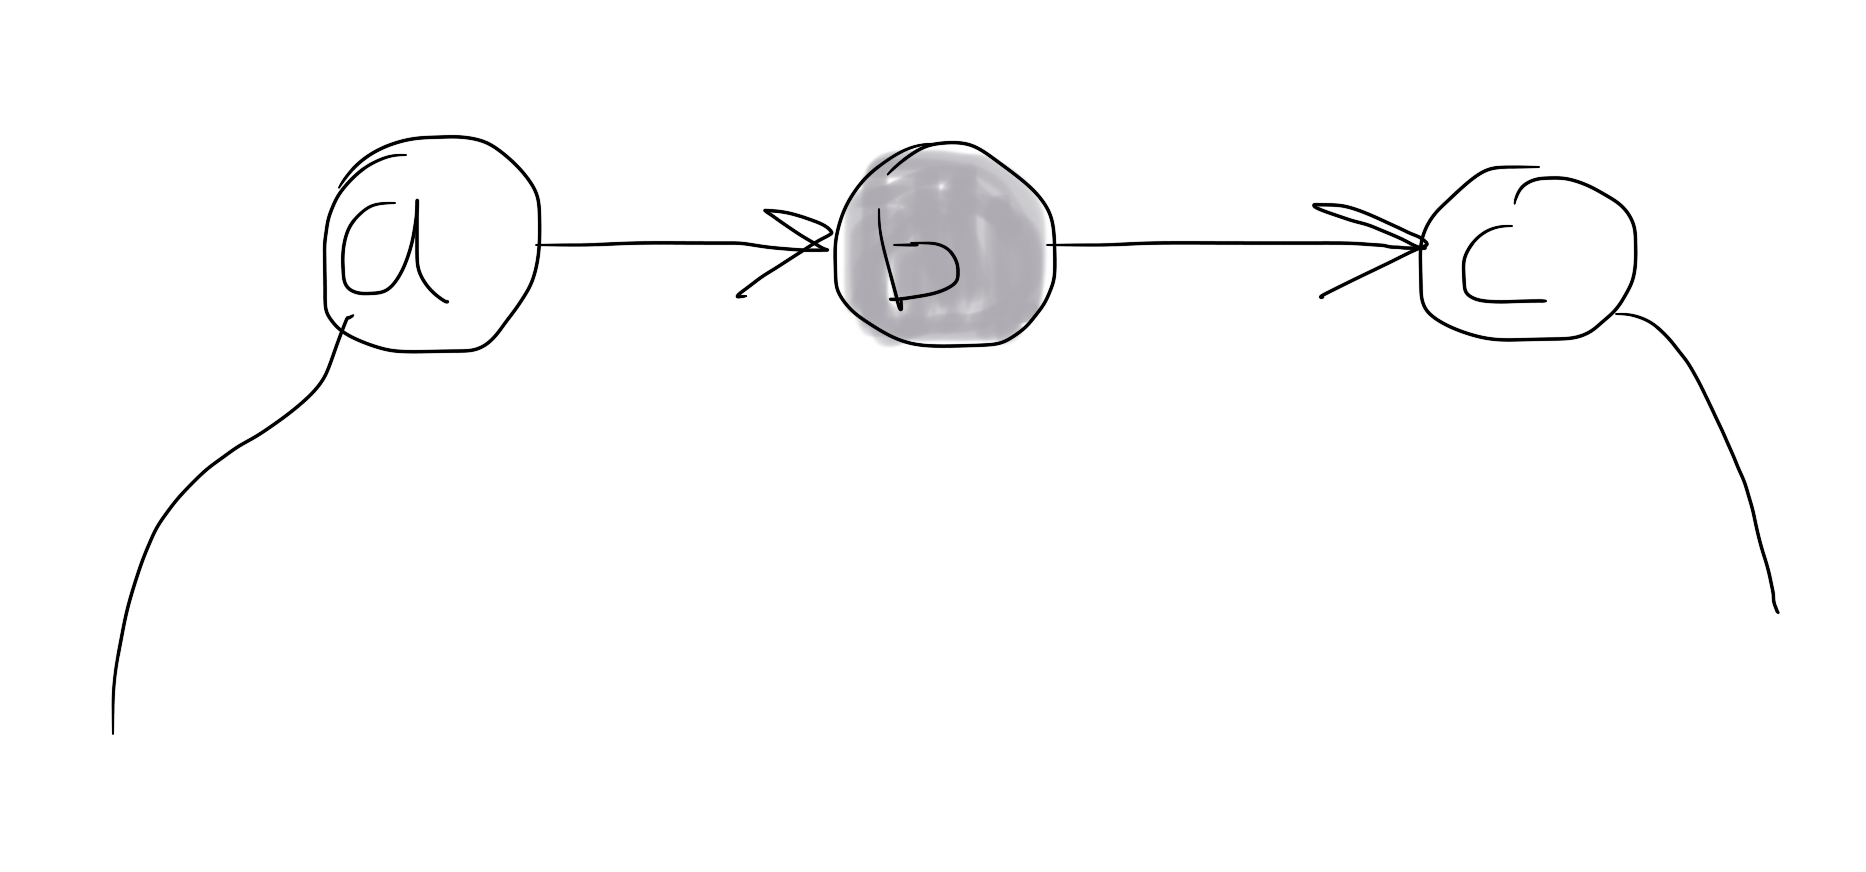
\includegraphics[scale=0.07]{imgs/img4.png}
	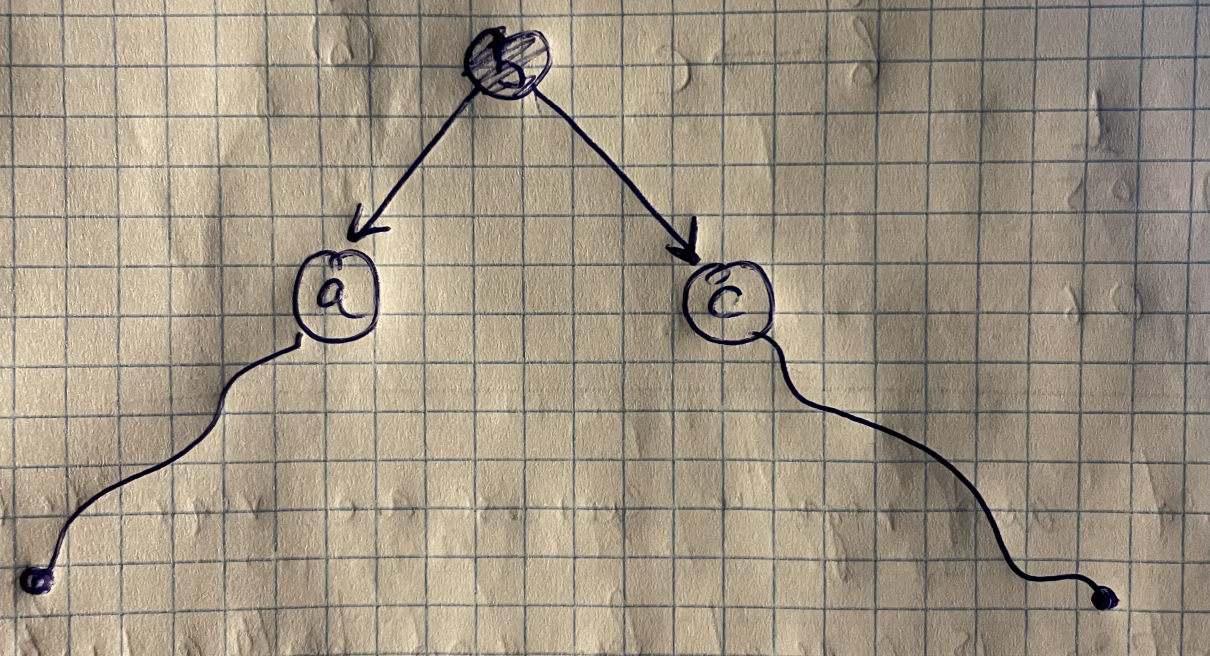
\includegraphics[scale=0.07]{imgs/img5.png}
	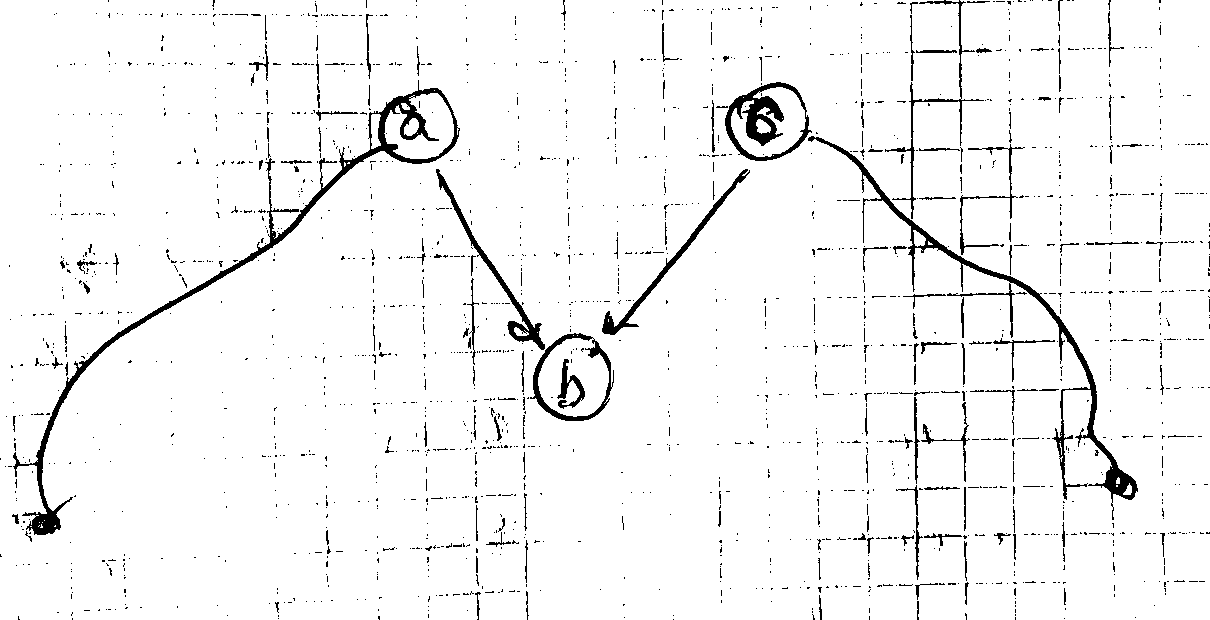
\includegraphics[scale=0.08]{imgs/img6.png}
\end{center}
	\caption{Различные причины $d-$сепарации, заштрихованные вершины $\in Z$}
	\label{fig:dsep1}
\end{figure}

Множество $Z$ $d-$разделяет множества $X$ и $Y$, если оно блокирует любой путь между $X$ и $Y$.

\subsection*{Приложения d-разделения}

А зачем собственно мы вводили $d-$разделение? А вот зачем:

\begin{theorem} Вероятностные следствия $d-$сепарации\\
Если множества $X$ и $Y$  d-разделены множеством $Z$, то $X \independent Y\ |\ Z$ в любом распределении, совместимом с $G$. Обратно, если $X$ и $Y$ не d-разделены $Z$ в $G$, то существует как минимум одно распределение, согласованное с $G$: $X \not \independent Y \ | \ Z$ в нем.
\label{th:th1}
\end{theorem}

Пруф: Начнем с введения понятия отношения полуграфоида.

\vspace{0.2cm}

\define{Модель зависимостей} - это тернарное отношение над множеством подмножеств $2^V$ некоторого множества $V$, тройки которого интерпретируются как утверждения о независимости первого и третьего элемента при условии, что известен второй.

\define{Полуграфоид (semi-graphoid)} - это замыкание модели зависимостей относительно первых четырёх свойств ($X, Y, Z, W$ - непересекающиеся подмножества множества-носителя $V$):
\begin{tcolorbox}
1. Симметрия: $I(X, Z, Y) \iff I(Y, Z, X)$ \\
2. Декомпозиция: $I(X, Z, Y\cup W) \implies I(X, Z, Y)\ \&\ I(X, Z, W)$\\
3. Слабое объединение: $I(X, Z, Y\cup W) \implies I(X, Z \cup W, Y)$\\
4. Сокращение: $I(X, Z\cup Y, W)\ \&\ I(X, Z, Y) \implies I(X, Z, Y\cup W)$\\
5. Пересечение: $I(X, Z\cup Y, W)\ \&\ I(X, Z\cup W, Y) \implies I(X, Z, Y\cup W)$
\end{tcolorbox}

Если кроме того полуграфоид замкнут относительно ещё пятого свойства, то он называется \textbf{графоидом}.


Примером полуграфоида (собственно, почему они нам в данном контексте интересны), заданным на множестве подмножеств случайных переменных $V$, будет отношение условной независимости: $I(X,Y,Z) \iff X \independent Y\ |\ Z$. Если распределение к тому же является строго положительным, то есть для любого набора значений переменных $(x_1...x_N):\ \forall i \in [1..N]\ \sum\limits_{X_j, j\neq i}P(x_1, ..., x_N) > 0 \implies P(x_1..X_N) > 0$, то отношение условной независимости будет графоидом. Почему важно это условие? Рассмотрим, когда будем пруфать свойство 5.

\vspace{0.2cm}
Давайте это докажем, чтобы просто поразминаться.

1. Весьма очевидно: действительно, если $P(X, Y | Z) = P(X | Z)P(Y|Z)$, то и симметричное верно, так как $P(Y,X|Z) = P(X,Y|Z) = P(X|Z)P(Y|Z) = P(Y|Z)P(X|Z)$.

2. Пусть $P(X, YW | Z) = P(X|Z)P(YW|Z) $. Тогда просто просуммируем правую и левую часть по множеству значений $W$:\\
Для левой части имеем $\sum\limits_{w}P(X,YW|Z) = P(X,Y|Z)$.\\
Для правой части аналогично 

\begin{align}
	\sum\limits_{w}P(X|Z)P(YW|Z) = P(X|Z)\sum\limits_{w}P(YW|Z) = P(X|Z)P(Y|Z)
\end{align} 
предпоследний переход в силу $Z \cap W = \emptyset$.

По условию левая и правая часть равны, значит $P(X,Y|Z) = P(X|Z)P(Y|Z)$. 

3. Пусть $P(X,YW|Z) = P(X|Z)P(YW|Z)$. Тогда по свойству декомпозиции 

\begin{align}
	P(X,W|Z)=P(X|Z)P(W|Z)
	\end{align}

Запишем факторизацию 
\begin{align}
	P(X,Y,Z,W) = P(X,YW|Z)P(Z) = P(X|Z)P(YW|Z)P(Z)=P(X|Z)P(Y|ZW)P(W|Z)P(Z)
\end{align}

\begin{align}
	\begin{split}
	P(X,Y|ZW) &= \frac{P(X,Y,Z,W)}{P(Z,W)} = \frac{P(X|Z)P(Y|ZW)P(W|Z)P(Z)}{P(ZW)} = \frac{P(X,W|Z)P(Y|ZW)P(Z)}{P(ZW)} \\
	&= \frac{P(X,Z,W)P(Y|ZW)}{P(ZW)} = P(X|ZW)P(Y|ZW)
\end{split}
\end{align}

4. Пусть 
\begin{align}
	P(X,W|ZY) &=P(X|ZY)P(W|ZY)\\
	P(X,Y|Z) &= P(X|Z)P(Y|Z)
\end{align}

Рассмотрим $P(X,YW|Z)$:

\begin{align}
	\begin{split}
	P(X,YW|Z)&= \frac{P(X,Y,Z,W)}{P(Z)} = \frac{P(X,W|ZY)P(ZY)}{P(Z)} = \frac{P(X|ZY)P(W|ZY)P(ZY)}{P(Z)}\\
	&= P(X|ZY)P(W|ZY)P(Y|Z) = P(X|ZY)P(Y,W|Z) = \frac{P(X,Y|Z)}{P(Y|Z)}P(Y,W|Z) \\
	&= \frac{P(X|Z)P(Y|Z)}{P(Y|Z)}P(Y,W|Z) = P(X|Z)P(YW|Z)
	\end{split}
\end{align}

5. Пусть
\begin{align}
	P(X,W|Z,Y) &= P(X|Z,Y)P(W|Z,Y)\\
	P(X,Y|Z,W) &= P(X|Z,W)P(Y|Z,W)
\end{align}

Умножим первое тождество на $P(Y)$, второе на $P(W)$:

\begin{align}
	P(X,W,Y|Z) &= P(X|Z,Y)P(W|Z,Y) P(Y) = P(X|Z,Y)P(W,Y|Z)\label{eq:fifth}\\
	P(X,Y,W|Z) &= P(X|Z,W)P(Y|Z,W) P(Y) = P(X|Z,W)P(Y,W|Z)
\end{align}

Приравняв правые части, и используя свойство положительности (вот тут оно нужно), сократим на $P(Y,W|Z)$, получаем
\begin{align}
	P(X|Z,Y) = P(X|Z,W)
\end{align}
Видим, что правая часть не зависит от $Y$, значит и левая не должна зависеть: $P(X|Z,Y) = P(X|Z)$. Аналогично $P(X|Z,W) = P(X|Z)$.
Нам же надо показать, что $P(X,Y,W|Z) = P(X|Z)P(Y,W|Z)$. можно заметить, что это следует из \ref{eq:fifth}, если использовать независимость $X \independent Y\ | \ Z$, выведенную ранее.

Ну в общем, вроде всё верно :) Более интересно, что эти свойства достаточны, чтобы определить все свойства вероятностной независимости.

Теперь перейдём к тому, как задать модель зависимостей на данном множестве. Понятно, что можно поступить наивным образом и задать её явно, перечислив список троек $(X, Z, Y)$, для которых отношение независимости выполняется. Однако, этот список будет в общем случае расти экспоненциально с ростом размера множества-носителя, так как экспоненицально растёт число различных его подмножеств. Представление модели зависимостей в виде графа, в свою очередь, может быть интуитивно понятным, компактным, а также с графами можно эффективно работать.

Есть как водится два основных варианта: использовать \textbf{неориентированные} и \textbf{ориентированные} графы.

В случае \textbf{неориентированных} графов, интерпретация довольно простая: элементам множества ставятся в соответствие вершины, и множества вершин $X$ и $Y$ независимы при условии $Z$, если оно разделяет $X$ и $Y$ в обычном смысле теории графов, то есть если любой путь $X$ в $Y$ обязательно содержит хотя бы одну вершину из $Z$. 
Ну, тут стоит отметить, что вообще говоря далеко не любой полуграфоид в таком виде представим точно: в большинстве случаев в графе будут отсутствовать некоторые независимости. Например, если модель зависимостей над множеством из трёх элементов $V = \{x,y,z\}$ содержит единственную независимость
 $I(\{x\}, \{y\}, \emptyset)$, то никак соответствующий ей полуграфоид  (заметим: в полуграфоиде будут две независимости в силу симметрии) не представить, не добавив лишних зависимостей, либо не убрав имеющиеся независимости.
 
 На самом деле, множество полуграфоидов, которые точно задаются неориентированными графами - это замыкание намного более сильного класса свойств:
 \begin{tcolorbox}
 1. Симметрия: $I(X, Z, Y) \iff I(Y, Z, X)$ \\
 2. Декомпозиция: $I(X, Z, Y\cup W) \implies I(X, Z, Y)\  \&\ I(X, Z, W)$\\
 3. \textbf{Сильное} объединение: $I(X, Z, Y) \implies I(X, Z \cup W, Y)$\\
 4. Пересечение: $I(X, Z\cup Y, W)\ \&\ I(X, Z\cup W, Y) \implies I(X, Z, Y\cup W)$\\
 5. Транзитивность: $I(X,Z,Y) \implies I(X, Z, W) \lor I(Y, Z, W)\ \forall \ W:\ W \cap (X \cup Y \cup Z) = \emptyset$
 \end{tcolorbox}
 
 Ну то, что эти свойства верны для представлений в виде неориентированных графов, весьма понятно. Давайте докажем что отношение, замкнутое относительно этих свойств, является графоидом. По сути, три свойства графоидов совпадают в данном определении, так что вывести остаётся только два: слабое объединение и сокращение.
 
 Начнём со слабого объединения: $I(X,Z,Y\cup W) \implies I(X, Z, Y) \implies I(X, Z \cup W, Y)$, где первый переход в силу свойства декомпозиции, второй - в силу свойства сильного объединения.
 
 Докажем свойство сокращения:  $I(X, Z, Y) \implies I(X, Z\cup W, Y)$ в силу сильного объединения, а значит $I(X, Z\cup Y, W)\ \&\ I(X, Z, Y) \implies I(X, Z\cup Y, W)\ \&\ I(X, Z\cup W, Y) \implies I(X,Z,Y \cup W)$, где последний переход сделан в силу свойства пересечения. 

\vspace{0.2cm}

В общем понятно, неориентированные графы прикольные, но могут представить довольно ограниченное подмножество возможных моделей независимостей (тут и далее будем использовать этот термин как синоним полуграфоида, полагая, что модель зависимостей замкнута относительно свойств 1-4 полуграфоидов).

Вообще говоря, довольно часто нам не требуется идеальное представление модели зависимостей, а вполне достаточно разумного приближения, которое не будет содержать \textbf{все} независимости, определенные моделью, но по крайней мере не будет содержать лишние. Такое представление назовём \textit{I-map} (от \textit{independence}).

Перейдём к представлению модели зависимостей в виде ориентированных графов, или, точнее, DAG. интерпретация таких графов проста: ребро означает непосредственную причинную зависимость двух переменных. Увы, простые разрезы графа в данном случае уже не будут отражать независимость, так как обуславливание на какое-то общее следствие двух несвязанных событий может сделать их зависимыми. Поэтому, вместо обычного разделения графа вводится понятие d-разделения (мы о нём уже говорили).

\define{Хвостовая граница (\textit{tail boundary})} переменной $x$ - это подмножество $B$ множества переменных $L$ меньших $x$ в смысле некоторого полного порядка на множестве переменных такое, что $I(x,B, L \backslash B)$.

\define{Протокол стратификации} $L_\theta = (\theta, B(x))$ это пара из полного упорядочивания переменных $\theta$, и функции $B(x)$ отображающей переменную на её хвостовую границу.

По протоколу стратификации однозначно строится DAG  очевидным образом. Ясно, что для заданной модели зависимостей на $n$ переменных существует $n!$ полных упорядочиваний. Для каждого полного упорядочивания в худшем случае существует $2^{n(n-1)/2}$ различных способов задать хвостовые границы (для каждой переменной все предыдущие в худшем случае могут как присутствовать в границе, так и нет $\implies$ для переменной номер $i$ может оказаться $2^{i-1}$ различных функций, задающих хвостовую границу). Итого, может существовать до $n!2^{\frac{n(n-1)}{2}}$ разных протоколов стратификации для заданной модели зависимостей.

Утверждается, что если модель зависимостей обладает идеальным представлением в виде DAG (то есть существует такой DAG, в котором есть все независимости из модели, и только они, или что то же самое, он является и I-map и D-map одновременно), то один из протоколов стратификации его задаёт. Докажем это.

Рассмотрим граф $D$, идеально представляющий модель. Он задаёт частичный порядок на множестве переменных $\phi$. Пусть $\theta$ - любо полный порядок, согласованный с $\phi$. Тогда $L = (\theta, Par(x))$ будет определять протокол стратификации, генерирующий $D$ (нетрудно увидеть, что непосредственные родители $x$ являются хвостовой границей).
$\blacksquare$ 

Если существует идеальное представление модели в виде DAG, то его можно найти, однако проверка на существование - это в общем случае сложная задача. Практически часто достаточно найти минимальный I-map, и следующая теорема покажет, что для любого полуграфоида (не обязательно имеющего идеальное представление в DAG) можно использовать стратификационные протоколы для построения I-map.

\begin{theorem} Если $M$ - полуграфоид, и $L_\theta$ - любой его протокол стратификации, то DAG, сгенерированный по этому протоколу, будет I-map полуграфоида.
\end{theorem}

Пруф по индукции по числу переменных в модели. Понятно, что для модели из одной переменной существует единственный DAG, и он конечно является I-map. Пусть теперь утверждение верно для моделей с числом переменных меньше $k$. Пусть $M$ имеет $k$ переменных, и имеется её протокол стратификации $L_\theta$, последняя по порядку $\theta$ переменная $n$, $M-n$ - полуграфоид, полученный удалением всех отношений независимости, содержащих переменную $n$, $G-n$ - DAG с удалённой вершиной $n$  и всеми инцидентными ей рёбрами. $n$- последняя переменная в упорядочивании, поэтому она не содержится ни в какой хвостовой границе из протокола $L_\theta$, так что $L_\theta - n$ (это $L_\theta$ с удаленным правилом для переменной $n$) будет протоколом стратификации для $M-n$. Графом, который генерирует $L_\theta-n$, будет $G-n$, и по индукции он является I-map $M-n$. 

Обозначим $M_G$ модель зависимостей, построенную по $G$ (то есть с использованием всех возможных d-разделений в графе), $M_{G-n}$ - соответственно модель,, сгенерированная по $G-n$. Сайд-ноут: по идее $M_G$ может содержать больше независимостей, чем есть $d-$разделений в $G$, так как оно строится как замыкание всех независимостей, полученных из $G$, но кажется нам бы доказать, что там нет лишних независимостей (об этому будет лемма ниже). По индукции, как сказано выше, $M_{G-n} \subset M-n$. Соответственно, нам надо показать, что $M_{G} \subset M$. Любая тройка $T \in M_G$ может быть отнесена к одной из четырёх непересекающихся категорий: либо $n$ не представлено ни в одном из трёх множеств, составляющих $T$, либо $n$ в каком-то из этих трёх множеств.

\textbf{Лемма} Пусть G - DAG, и $M_G$ - модель зависимостей, индуцированная им. Тогда G - идеальное представление $M_G$ в виде DAG.
Заметим, G является I-map для $M_G$, так как все независимости из $G$ по построению имеются в $M_G$. Значит, остаётся показать, что G - D-map. Для этого нужно доказать, что в G выполняются свойства 1-4 полуграфоидов (ведь тогда d-разделенные тройки замкнуты в G, а значит в $M_G$).

1. Свойство симметрии выполняется очевидно (если $X \indepg Y \ | \ Z \implies Y \indepg X \ | \ Z$)

2. Свойство декомпозиции в общем тоже очевидно верно: если $Z$ блокирует пути между $X$ и $Y\cup W$, то конечно $Z$ блокирует пути между $X$ и $Y$.

3. Свойство слабого объединения: пусть $X \indepg Y\cup W | Z$. Надо показать, что $X \indepg Y | Z \cup W$. Будем рассуждать от противного, пусть не так. Заметим, что по свойству декомпозиции, $X \indepg Y | Z$ и $X \indepg W | Z$. Значит, добавление к $Z$ множества $W$ разблокировало какой-то путь между $X$ и $Y$. Но это возможно, только если разблокированный путь $X \leadsto Y$ имеет v-структуру с концом в $W$, то есть $X\leadsto...\rightarrow w \leftarrow ...\leadsto Y$, где $w \in W$. Ясно, что при этом путь $X\leadsto w$ разблокирован. Рассмотрим аналогично этот путь (он будет короче предыдущего). Он либо был разблокирован до обуславливания на $W$, либо стал таким после. Во втором случае мы повторяем логику и откусываем опять префикс пути, повторя подход пока не окажемся в первом случае. В первом же случае, у нас префикс пути до $w$ не заблокирован при обуславливании на $Z$, но тогда $X \not \indepg w | Z$, что противоречит исходному предположению.

4. На десерт, свойство сокращения. Пусть $X \indepg W | Z\cup Y$ и $X \indepg | Z$. Нам надо показать, что $X\indepg Y \cup W | Z$. 

Ну, начнём с того, что по условию, $Z$ блокирует все пути $X \leadsto Y$. Значит, нам остаётся показать, что $Z$ блокирует все пути $X \leadsto W$. Предположим, это не так. Тогда существует незаблокированный путь $p = X \leadsto W$. заметим, что по условию $Z \cup Y$ отделяет $W$ от $X$, значит $Y$ должно блокировать путь $p$, а значит, $p = X\leadsto...\rightarrow y \rightarrow ... W$ или $p = X \leadsto ... \leftarrow y \rightarrow ... \leadsto W$, где $y \in Y$, причем префикс пути $p$ вплоть до $y$ не блокируется $Z$ (иначе путь был бы заблокирован и без обуславливания на $y$). Но это в свою очередь означает, что существует незаблокированный путь от $X$ до $y$, что противоречит тому, что $Z$ d-разделяет $X$ и $Y$. 
$\blacksquare$ 

В общем, теперь показано, что $(X, Z, Y) \in M_G \iff X \indepg Y | Z$, то есть отношение d-сепарации задаёт графоид на DAG.

\textbf{Кейс 1}: $n$ не представлено в $T = (X, Z, Y)$. $T \in M_G \implies T \in M_{G-n}$, так как иначе в $G-n$ существует незаблокированный множеством $Z$ путь, но тогда этот же незаблокированный путь есть и в $G$, так как добавление вершин и рёбер не может заблокировать путь. $G-n$ - I-map для $M-n$, значит $T \in M-n$, и так как $M-n \subset M$, то $T \in M$.

\textbf{Кейс 2}: $T=(Xn, Z, Y)$. Пусть $(n, B, R) \in L_\theta$ - последний триплет протокола стратификации (и конечно единственный, содержащий $n$), $B = B_X \cup B_Y \cup B_Z \cup B_0$, $R = R_X \cup R_Y \cup R_Z \cup R_0$, причём $X = B_X \cup R_X$, $Y = B_Y \cup R_Y$, $Z = B_Z \cup R_Z$ \ref{fig:case2}.

\begin{figure}[h]
	\begin{center}
		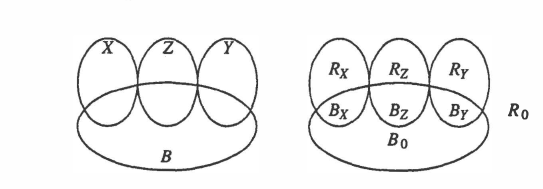
\includegraphics[scale=0.6]{imgs/img7.png}
	\end{center}
	\caption{Кейс 2}
	\label{fig:case2}
\end{figure}

По построению, из всех вершин $B$ есть ребро в $n$. Раз $T \in M_G$, то любой путь между $n$ и $Y$ должен быть заблокирован $Z$, поэтому $B_Y = \emptyset$, иначе был бы путь, состоящий просто из одного ребра, из $b \in B_Y$ в $n$. Таким образом, $Y = R_Y$, и последний триплет протокола представим в виде $(n, B_XB_0B_Z,R_XR_ZR_0Y)$.

Так как $M$ полуграфоид,то по свойству слабого объединения мы можем перенести $R_XR_Z$ из третьего элемента триплета во второй и получить корректное отношение независимости: $(n, BRB_0, YR_0) \in M$. Также, в силу декомпозиции, можем забить в последнем элементе тройки на $R_0$ и снова получить элемент $M$: 
\begin{align}
	(n, XZB_0, Y) \in M
	\label{eq:case2}
\end{align}

Все элементы $B_0$ соединены ребром с $n$, и $n$ d-отделено от $Y$ вершинами $Z$, значит $B_0$ тоже d-отделено от $Y$ тем же $Z$, так как иначе существовал бы путь $B_0 \leadsto Y$, но тогда в силу того что из $B_0 \rightarrow n$, был бы незаблокированный $Z$ путь $Y \leadsto n$. Теперь, раз $X$ и $B_0$ d-разделены  c $Y$ через $Z$, то и их объединение тоже отделено от $X$ через $Z$, так что $(XB_0, Z, Y) \in M_G$. В этой тройке не фигурирует $n$, значит по кейсу 1 имеем $(XB_0, Z, Y) \in M$. Объединяя это с \ref{eq:case2} и используя свойство сокращения, получаем $(Y, Z, nXB_0) \in M$, а тогда по свойству декомпозиции $(nX, Z, Y) \in M$. 

\textbf{Кейс 3}: $T = (X,nZ,Y)$. Опять представим последний элемент протокола стратификации в виде $(n, B_XB_YB_ZB_0, R_XR_YR_ZR_0 \in M$.  Заметим, что $B_X = \emptyset \lor B_Y=\emptyset$, так как иначе есть путь $b_x\rightarrow n \leftarrow b_y$, разблокированный обуславливанием на $n$, то есть был бы незаблокированный путь $X \leadsto Y$, а это бы противоречило тому, что $T \in M_G$. Не умаляя общности, пусть $B_Y = \emptyset$. По соображениям из предыдущего пункта, $(B_0,Z,Y) \in M_G$.

Далее, $(X, nZ, Y) \in M_G \implies (X, Z, Y) \in M_G$, так как $n$ имеет только входящие рёбра, а значит, если бы был незаблокированный $Z$ путь $X \leadsto Y$, то обуславливание на $n$ не помогло бы его заблокировать. Значит, $(XB_0, Z, Y) \in M_G$, и по кейсу 1 также $(XB_0, Z, Y) \in M$. По рассуждениям из кейса 2, последний триплет протокола представим в виде $(n, B_XB_0B_Z,R_XR_ZR_0Y) \in M$  и в итоге $(n, XZB_0, Y) \in M \implies (nXB_0, Z, Y) \in M \implies (XB_0,nZ,Y) \implies (X,nZ,Y)$ (слабое объединение, затем декомпозиция).

\textbf{Кейс 4}: $T = (X,Z,nY)$ - засчёт симметрии сводится к кейсу 2.
$\blacksquare$

 \begin{tcolorbox}
По смыслу, как юзать эту теорему, то есть какие следствия? А вот какие: допустим есть модель зависимостей (любой полуграфоид), и мы построили для неё какой-то протокол стратификации $L_\theta$, а по протоколу стратификации построили DAG. Так вот, тогда любое d-разделение множеств в DAG означает принадлежность соответствующей тройки (условную независимость) в модели зависимостей.
\end{tcolorbox}

Ещё одно простое следствие: если протокол стратификации модели зависимостей $M$ $L_\theta$ таков, что все хвостовые границы в нём минимальны (нельзя удалить элемент ни из одной с тем чтобы не нарушить принадлежность триплета $M$), то построенный по этому протоколу DAG является минимальным I-map модели - очевидно, он I-map по теореме, а минимальный, потому что каждое ребро определяется какой-то хвостовой границей протокола, значит никакое ребро нельзя удалить без нарушения I-map (иначе мы бы восстановили по усечённому DAG обратно урезанный протокол стратификации и он был бы корректен).

Возвращаясь к изначальной теореме, о следствиях d-разделения в контексте вероятностных распределений: мы показали, что если $P(V)$ марковское относительно DAG $G$ то $X \indepg Y | Z \implies X \independent Y | Z$. Ну, потому что в данном случае $P(V)$ выступает как модель зависимостей, а марковская согласованность позволяет построить протокол стратификации этой модели, соответствующий $G$. Но вот со вторым утверждением теоремы пока ничего не было сделано: что если в графе нет d-разделения множеств $X, Y$ посредством множества $Z$, то существует распределение, согласованное с G, в котором $X \not\independent Y | Z$. Пока оставим этот факт недоказанным.

\begin{theorem} \textbf{Условие упорядоченной марковости}\\
Необходимым и достаточным условием того, чтобы распределение $P$ было марковски согласованным с G является то, что каждая переменная независима от всех своих предшественников в некотором упорядочивании, согласованном с G при обуславливании на её родителей в G. 
\label{th:ordered_markov}
\end{theorem}

\textbf{Необходимость}: пусть P совместимо с G. Это значит, что $P(x_1..x_n) = \prod P(x_i|pa_i)$. Упорядочим переменные, используя топологическую сортировку согласно графу G. Нам надо показать, что $P(x_i | pa_i, x_j) = P(x_i | pa_i)$.

Заметим, что 
\begin{align}
	P(x_1...x_n) = \prod\limits_{k\le i}P(x_k|pa_k)\prod\limits_{k> i} P(x_k | pa_k)
	\label{eq:factorization1}
\end{align}

Отсюда легко выводится частное распределение первых $i$ переменных в выбранном нами порядке путём суммирования равенства

 \begin{align}
 	\begin{split}
 	P(x_1...x_i) &= \prod\limits_{k\le i}P(x_k|pa_k)\sum\limits_{x_j: j > i}\prod\limits_{k> i} P(x_k | pa_k)\\
 	&= \prod\limits_{k\le i}P(x_k|pa_k)\sum\limits_{x_j : i < j < n}\prod\limits_{ i < k < n}P(x_k | pa_k) \sum\limits_{x_n}P(x_n | pa_n)\\
 	&= \ldots = \prod\limits_{k\le i}P(x_k|pa_k)
 	\label{eq:factorization2}
 	\end{split}
 \end{align}

Используя \ref{eq:factorization2}, легко выводим соотношение

\begin{align}
	P(x_i|x_1,...,x_{i-1}) = \frac{P(x_1,...,x_i)}{P(x_1,...,x_{i-1})} = \frac{\prod\limits_{k\le i}P(x_k|pa_k)}{\prod\limits_{k\le i - 1}P(x_k|pa_k)} = P(x_i|pa_i)
\end{align}

Таким образом, $X_i \independent \{x_1...x_{i-1}\} \backslash PA_i\ |\ PA_i$. Мы уже ранее доказывали, что отношение условной независимости для множества случайных переменных образует графоид, а потому по свойству декомпозиции $\forall j < i: X_j \notin PA_i  \implies X_i \independent X_j | PA_i$, что собственно и требовалось.

\textbf{Достаточность}: пусть каждая переменная $X_i$ независима от всех переменных с меньшим номером при обуславливании на непосредственных предков переменной в графе G. Покажем, что в таком случае распределение марковски совместимо с G, то есть что оно факторизуется согласно G.

Любое распределение представим в виде следующей факторизации:
\begin{align}
	P(x_1,...,x_n) = \prod\limits_iP(x_i|x_1,...,x_{i-1})
\end{align}

Заметим, что теперь нам остаётся воспользоваться условием, что каждая переменная условно независима от всех переменных с меньшим номером при обуславливании на её родителей в графе G, чтобы получить необходимое равенство:

\begin{align}
	P(x_1,...,x_n) = \prod\limits_iP(x_i|pa_i)
\end{align}
$\blacksquare$

Ещё одна похожая теорема:

\begin{theorem} \textbf{Условие родительской марковости}\\
	Необходимым и достаточным условием того, чтобы распределение $P$ было марковски согласованным с G является то, что каждая переменная независима от всех своих \textit{не наследников} в некотором упорядочивании, согласованном с G при обуславливании на её родителей в G. 
\end{theorem}

\textbf{Необходимость}: пусть $P(v)$ совместимо с графом $G$, и $x_j \notin de(x_i)$. Покажем, что $x_i \independent x_j \ |pa_i$. Заметим, что если $j < i$, то утверждение вытекает из предыдущей теоремы об условии упорядоченной марковости. Пусть $j > i$. Ясно, что в графе $G$ не существует ни направленного пути $x_i \leadsto x_j$ (так как $x_j \notin de(x_i)$), ни направленного пути $x_j \leadsto x_i$, так как в таком случае упорядочение переменных было бы не согласовано с топологией графа. А значит, в любом пути, соединяющем $x_i$ и $x_j$, существует как минимум одно соединение вида $\rightarrow x_k \leftarrow$, и конечно $x_k \notin pa_i$, ведь тогда в неё не могло бы быть двух стрелок в пути. Но любой такой путь заблокирован множеством $pa_i$, значит $x_i$ и $x_j$ d-разделены в G множеством $pa_i$, а значит, условно независимы при обуславливании на $pa_i$ согласно вероятностным следствиям d-разделения.

\textbf{Достаточность}: тут всё просто, если каждая переменная независима от своих ненаследников, то она уж точно независима от всех переменных с меньшими, чем её, номерами, а значит по предыдущей теореме распределение согласовано с $G$.
$\blacksquare$

\define{Наблюдаемая эквивалентность} Два графа называют наблюдаемо эквивалентными, если любое распределение, согласованное с первым, согласовано со вторым, и наоборот.

\begin{theorem} \textbf{О наблюдаемой эквивалентности}\\
Два графа наблюдаемо эквивалентны тогда и только тогда, когда они имеют один и тот же скелет и набор $v-$структур. 
\end{theorem}

\textbf{Необходимость}: Пусть два графа наблюдаемо эквивалентны. Докажем, что у них один и тот же скелет и набор v-структур.

Начнём со скелета. Пусть в графе $G_1$ имеется ребро $x-y$, а в $G_2$ нет. Рассмотрим такое распределение:
\begin{align}
	P(x_1,..x_n) = uniform_{[0,1]}(x)bernoulli_x(y)
\end{align}

где все переменные, кроме двух рассматриваемых, константны. Заметим, что такое распределение будет согласованным с $G_1$, так как факторизуется согласно ему. В то же вермя, оно не согласованно с $G_2$. Действительно, пусть оно согласованно. Согласно теореме об упорядоченной марковости \ref{th:ordered_markov}, в этом случае существует согласованное с $G_2$ упорядочивание, при котором каждая переменная независима от переменных с меньшими номерами при обуславливании на её родителей в $G_2$. Не умаляя общности будем считать, что $x$ упорядочилась до $y$. Заметим, что $x \notin PA_y$, так как между ними нет ребра в $G_2$, а значит $P(y|x) = \sum\limits_{pa_y}P(y, pa_y|x) = \sum\limits_{pa_y}P(y|x,pa_y)P(pa_y|x) = \sum\limits_{pa_y}P(y|pa_y) = P(y)$, то есть $y$ должно быть независимо от $x$ в $P$, но это не так. Мы пришли к противоречию, значит $P$ несовместимо с $G_2$, но тогда $G_1$ и $G_2$ наблюдаемо неэквивалентны, что противоречит исходному предположению, значит, в $G_2$ тоже нет ребра $x-y$. Значит, скелеты графов совпадают.

Докажем теперь, что в графах совпадают v-структуры. Ну, это довольно просто доказать: рассмотрим любые такие два графа, и предположим, что утверждение ложно. Мы уже знаем, что скелеты графов совпадают, значит совпадают и неориентированные пути. Раз набор v-структур не совпадает,  существует как минимум один путь $x \leadsto y$, заблокированный $Z$ в первом графе, и не заблокированный во втором (симметричный кейс аналогичен). Рассмотрим этот путь в обоих графах. Разница в блокировке может быть связана только с различной ориентацией стрелок в какой-то вершине $v$. Существует всего четыре способа ориентации стрелок в пути: 

1. $...\rightarrow v \leftarrow ...$, но в таком случае $v$ имеет одинаковые стрелки в обоих графах, так как является вершиной v-структуры, значит эта вершина не может различать блокировку пути в графах.

2. $\rightarrow v \rightarrow$

3. $\leftarrow v \leftarrow$

4. $\leftarrow v \rightarrow$

Последние три вариант могут наблюдаться в обоих графах независимо. Однако, при любой комбинации, если $v \in Z$, то в обоих графах $v$ блокирует путь, а если $v \notin Z$, то не блокирует. То есть, в любом случае, любое допустимое направление стрелок в $v$  не может различать заблокированность пути в графах, значит предположение неверно.

\textbf{Достаточность}: пусть у двух графов одинаковый скелет и набор v-структур. Нам надо показать, что они наблюдаемо эквивалентны. 

Тут придётся немного попотеть. Доказывать будем по индукции по числу вершин в графах. С одной вершиной всё понятно верно, так что считаем, что база есть. 

Пусть мы доказали утверждение для всех графов с число вершин, меньшим $n$. Рассмотрим два графа на $n$ вершинах с одинаковым скелетом и набором v-структур. Предположим, что $P(v)$ согласованно с $G_1$, и покажем, что тогда оно согласовано и c $G_2$.

\begin{figure}[h]
	\begin{center}
		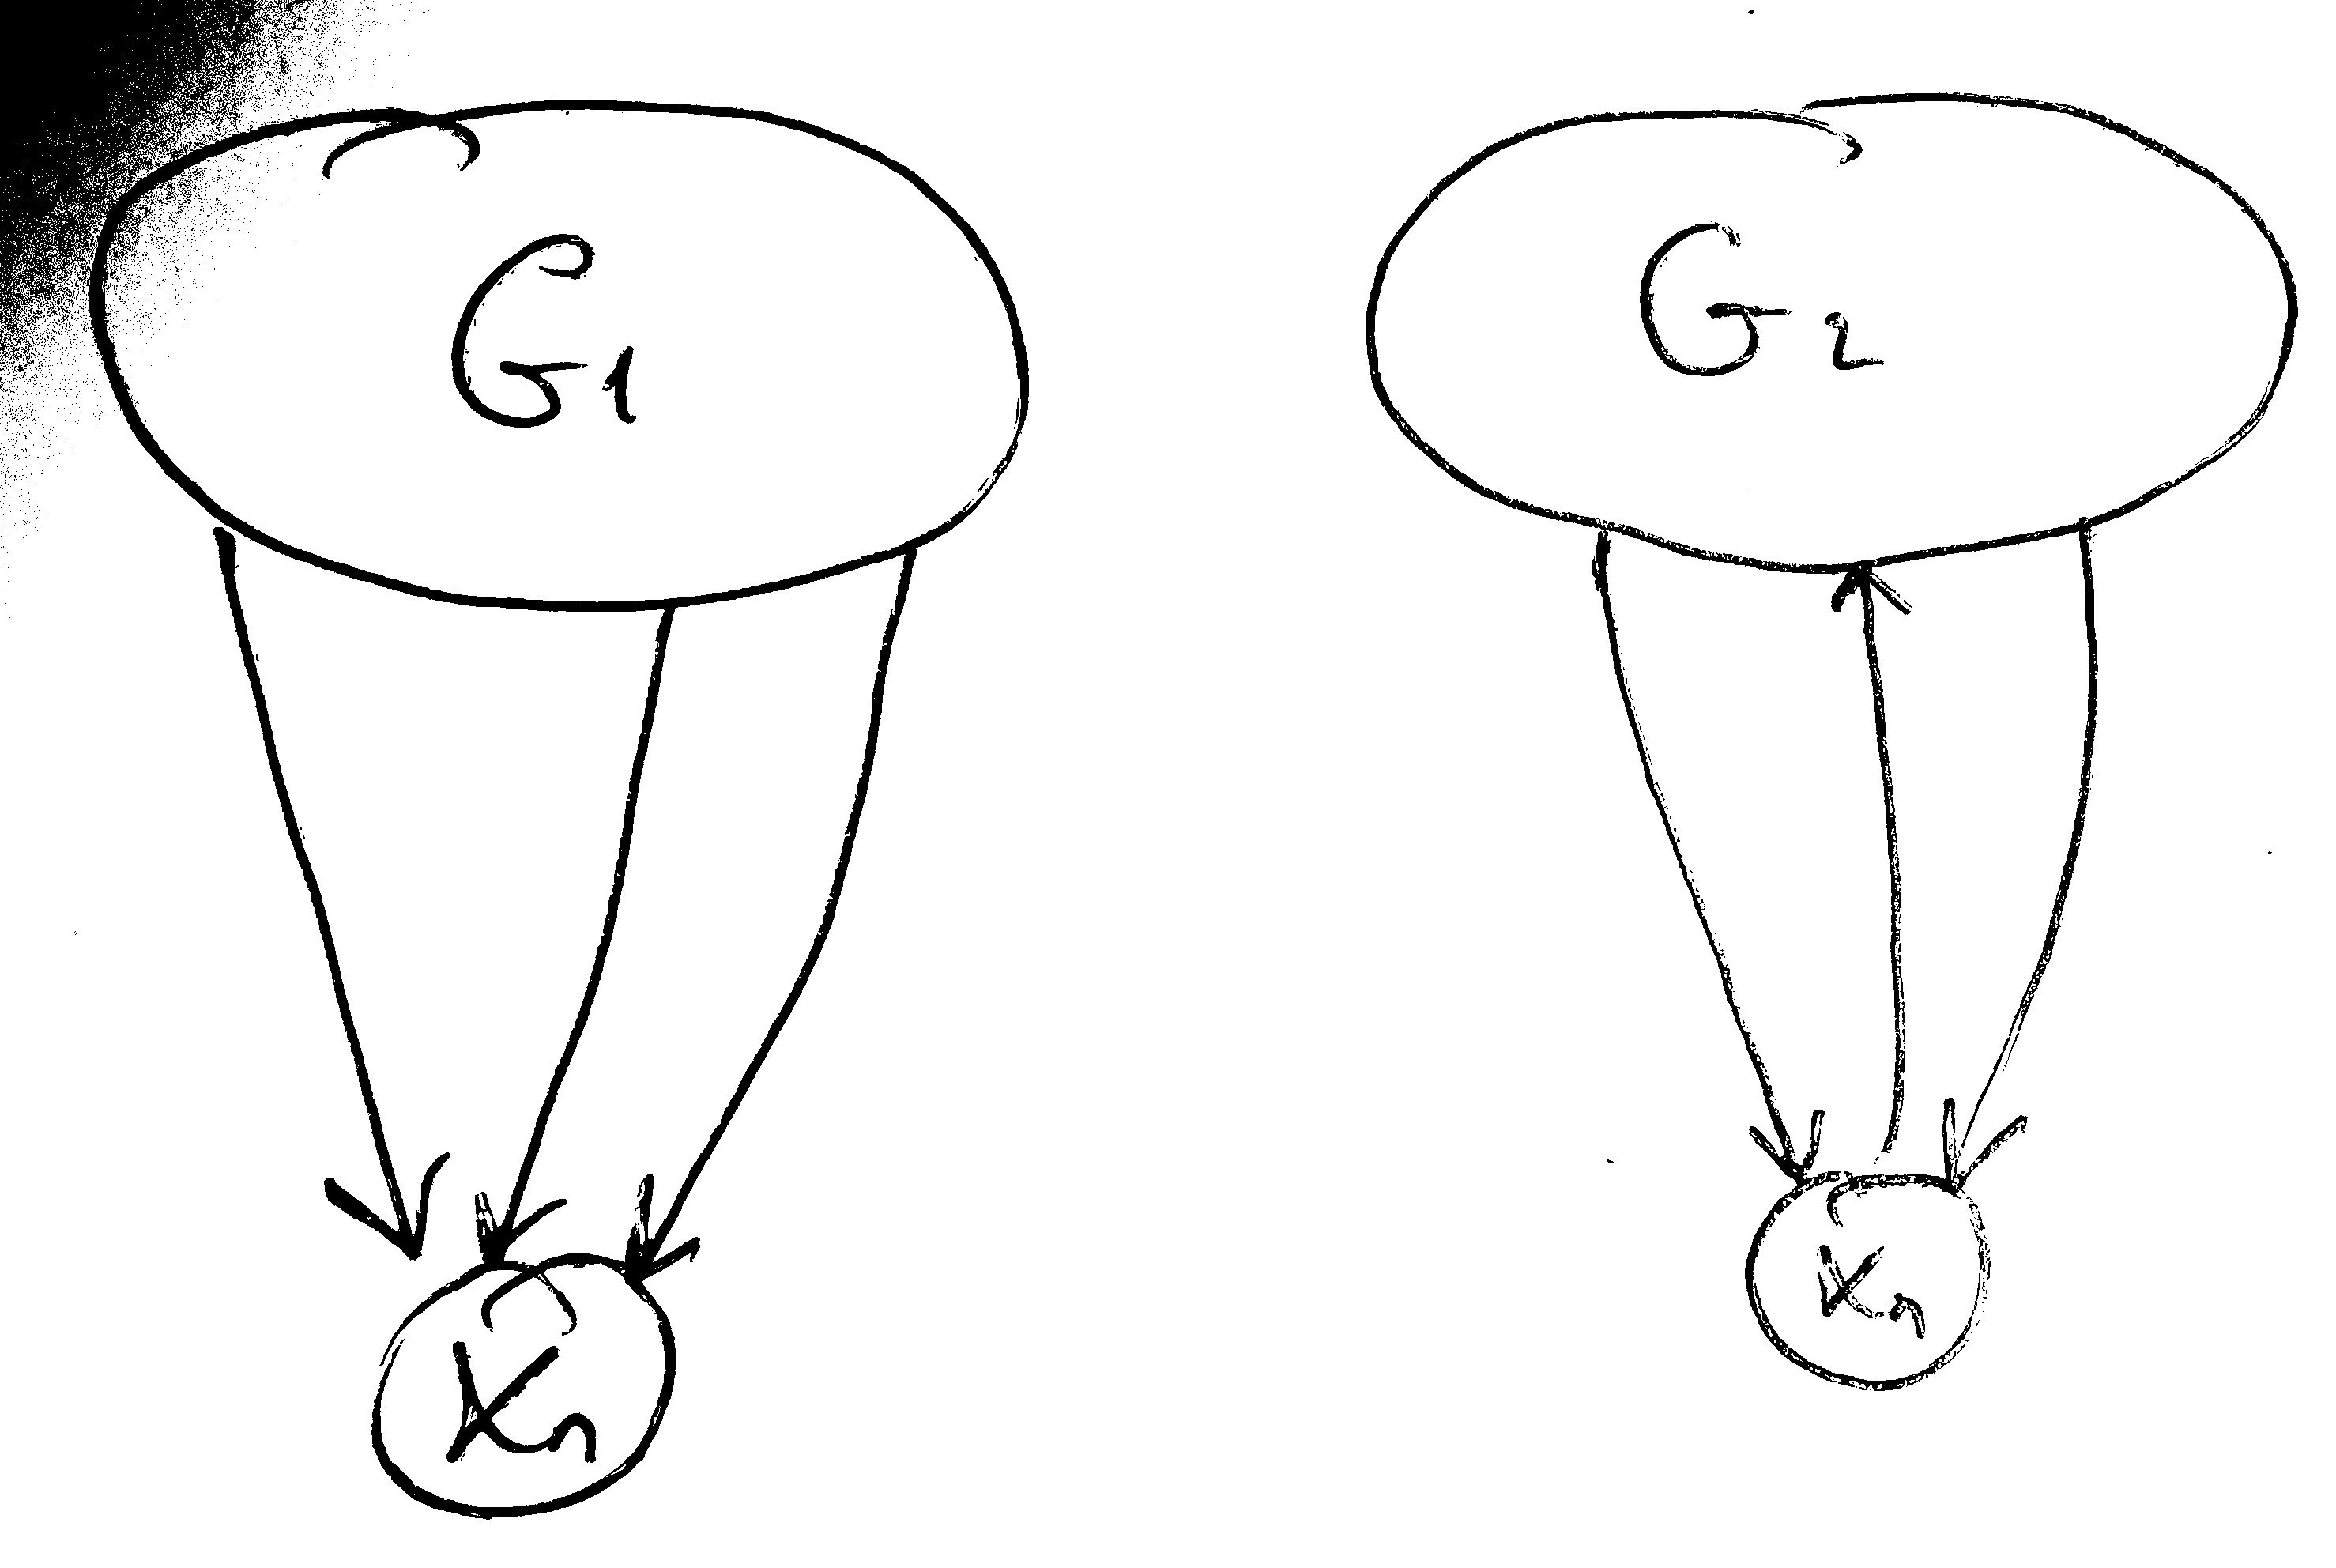
\includegraphics[scale=0.1]{imgs/img10.png}
	\end{center}
	\caption{Два рассматриваемых графа $G_1$ и $G_2$}
	\label{fig:equiv1}
\end{figure}

Раз $P(v)$ согласовано с $G_1$, то оно факторизуется согласно ему:

\begin{align}
	P(x_1,...x_n) = \prod\limits_{i}P(x_i|pa^1_{i})
\end{align}

Будем считать, что переменные упорядочены согласно топологии $G_1$, $pa^1_i$ - родители вершины $X_i$ в $G_1$. Аналогично, далее будем обозначать $pa^2_i$ - родители вершины $X_i$ в $G_2$. Понятно, что в общем случае $pa^1_i \neq pa^2_i$. 

Рассмотрим частное распределение  $P(x_1,..,x_{n-1})$. Оно  очевидно согласованно с $G_1-x_n$. Далее, заметим, что оно согласовано и с $G_2-x_n$, так как у этих двух графов на $n-1$ вершине одинаковые скелеты и v-структуры (скелеты понятно, а v-структуры - потому что мы не могли разрушить или добавить никакую v-структуру удалением $x_n$ из графа $G_2$, так как в $G_1$ эта переменная не участвует в формировании каких-либо v-структур, а значит аналогично и в $G_2$). Поэтому мы можем записать:

\begin{align}
	P(x_1,...x_{n-1}) = \prod\limits_{i}P(x_i|pa^1_{i}) = \prod\limits_{i}P(x_i|pa^2_{i} \backslash \{x_n\}) 
\end{align}

В последнем равенстве мы учитываем, что при удалении $x_n$ из $G_2$ некоторые вершины (а именно все, в которые из $x_n$ в $G_2$ ведёт ребро) из списка родителей вершины в графе $G_2-x_n$ приходится убирать $x_n$.

Перейдём обратно к полному распределению: 
\begin{align}
	P(x_1,...x_{n}) = P(x_1,...x_{n-1})P(x_n|pa^1_{n}) = \prod\limits_{i}P(x_i|pa^2_{i} \backslash \{x_n\}) P(x_n|pa^1_{n})
\end{align}

Разобьём мысленно множество $pa^1_n$ на три $pa^1_n = Q \cup R \cup S$

\begin{figure}[h]
	\begin{center}
		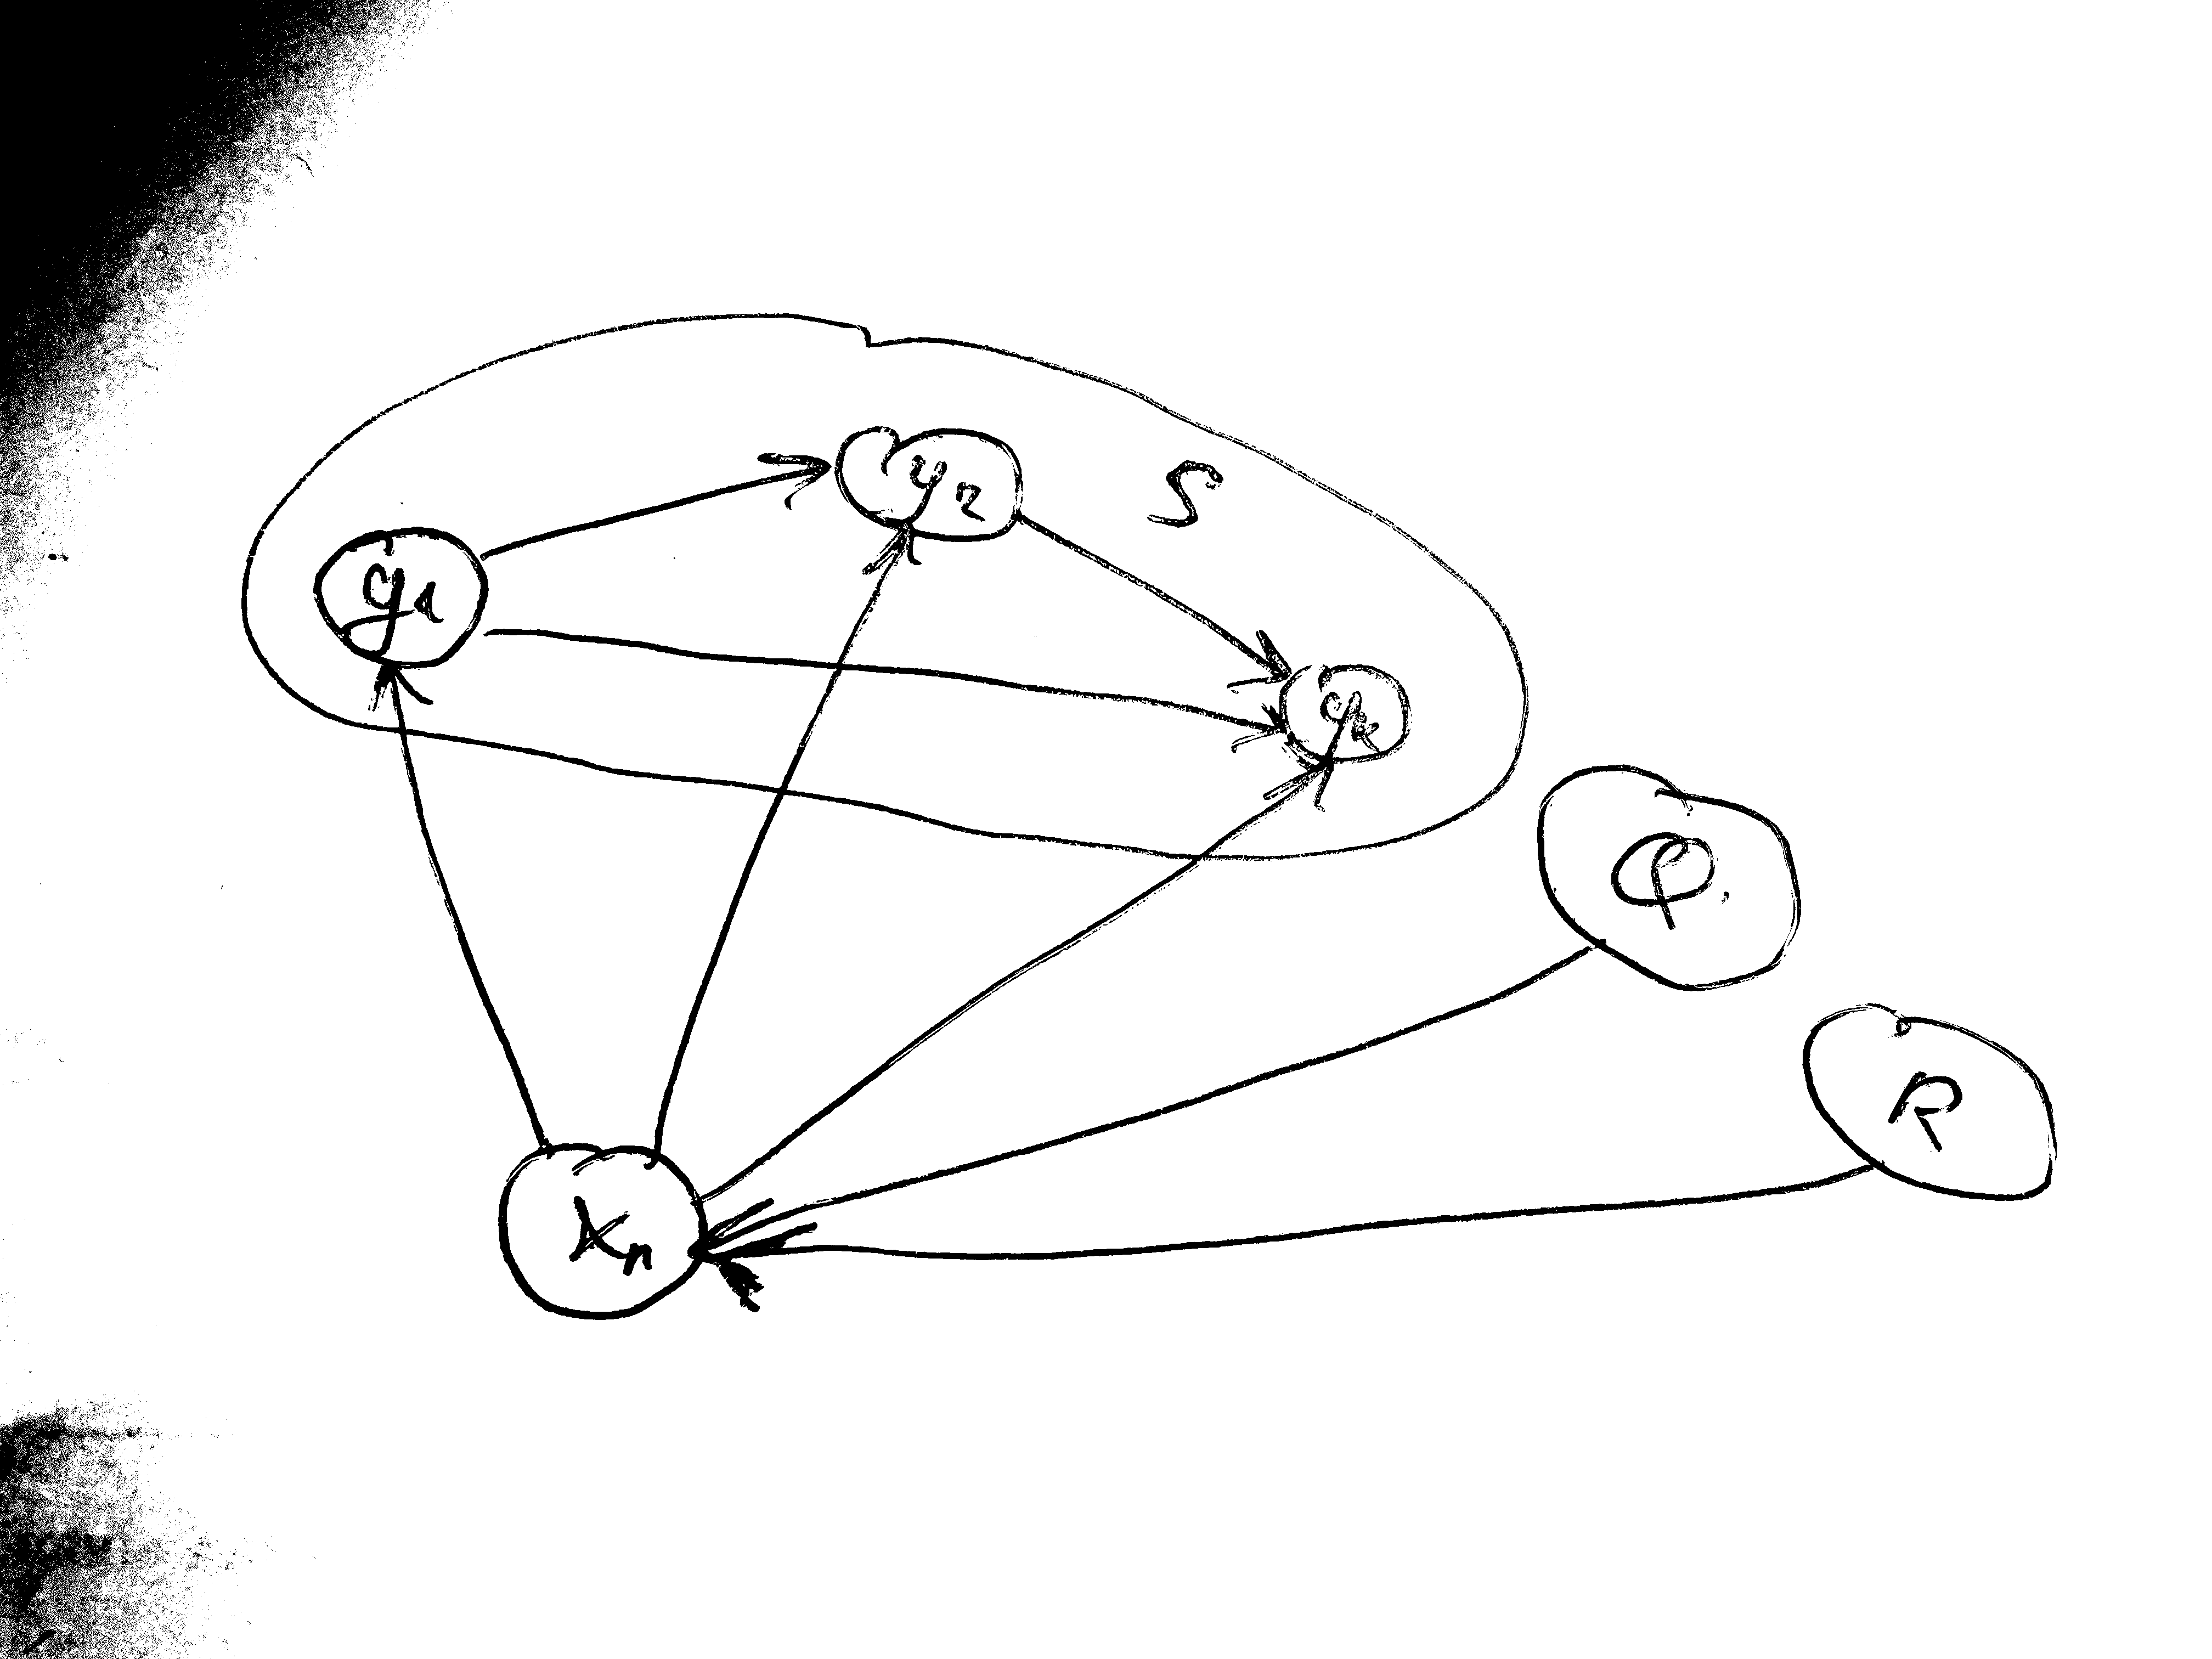
\includegraphics[scale=0.05]{imgs/img11.png}
	\end{center}
	\caption{Разбиение связанных с $x_n$ вершин на $Q,R,S$}
	\label{fig:equiv2}
\end{figure}


Здесь $Q$ - множество вершин, образующих v-структуру с $x_n$, то есть  $x_i, x_j \in Q \iff x_i \rightarrow x_n \leftarrow x_j$ и нет ребра, соединяющего $x_i$  с $x_j$. $R$ - множество вершин, из которых в $G_2$ есть ребро в $x_n$. $S$ - самое интересное множество, так как это множество вершин, ориентация рёбер между которыми и $x_n$ в $G_2$ инвертирована относительно $G_1$, то есть это все вершины, для которых в  $G_2$ вершина $x_n$ является родителем. Для наглядности, можно посмотреть на картинку \ref{fig:equiv2} 

Таким образом, $pa^1_n = Q \cup R \cup S$, $pa^2_n = Q \cup R$. Остановимся на множестве $S$: надо понять, что эти вершины образуют клику, то есть все они связаны рёбрами между собой. Действительно, если бы это было не так, то существовали бы две вершины $x_i, x_j \in S$: из $x_n$ есть в них ребро, но они не связаны между собой. Но тогда они в $G_1$ образовывали бы  v-структуру с вершиной в $x_n$, но тогда они согласно нашему разбиению бы оказались не в $S$, а в $Q$.  Тогда, мы можем представить факторизацию $P(v)$ следующим образом

\begin{align}
	P(x_1,...x_{n}) =  \prod\limits_{x_i\notin S}P(x_i|pa^2_{i})\prod\limits_{x_i\in S}P(x_i|pa^2_{i} \backslash \{x_n\}) P(x_n|Q, R)
	\label{eq:equiv1}
\end{align}

Пронумеруем вершины в $S$ в топологическом порядке в графе $G_2$. Ясно, что раз они все между собой связаны, это можно сделать единственным образом. Итак, пусть $S = \{y_1,y_2,...,y_k\}$. 
Заметим, что $pa^2_{y_j} \subset R \cup Q \cup \{y_1,...y_{j-1}\} \cup \{x_n\}$. Ну действительно, $y_{j+1},...y_{k}$ в родителях нет в силу того, что мы топологически пронумеровали вершины. Никаких прочих вершин $z$ там нет, так как если бы такая вершина была, то обязательно должно было бы присутствовать ребро $z \rightarrow x_n$, так как иначе $x_n \rightarrow y_j \leftarrow z$ образуют в $G_2$ v-структуру, которой нет в $G_1$, а значит $z \in Q \cup R$.

Нам надо показать, что $P(v) = \prod\limits_{i}P(x_i|pa^2_{i})$. Сравнивая с \ref{eq:equiv1}, приходим к тому, что надо показать

\begin{align}
	\prod\limits_{x_i\in S}P(x_i|pa^2_{i} \backslash \{x_n\}) P(x_n|Q, R, S) =  \prod\limits_{x_i \in S}P(x_i|pa^2_{i}) P(x_n|pa^2_n)
	\label{eq:equiv2}
\end{align}

Начнём сворачивать формулу в левой части, начиная со множителя для $y_k$ и $x_n$. Заметим, что $Q,R$ не содержат наследников $y_k$ в $G_2 - x_n$, иначе был бы цикл через $x_n$. Кроме того, $P(v\backslash \{x_n\})$ совместимо с $G_2 - x_n$ по предположению индукции. Значит, согласно теореме о родительском марковском условии, $P(y_k | pa^2_{y_k} \backslash \{x_n\}) = P(y_k|y_1,...y_{k-1},Q,R)$.

Тогда \begin{align}
	\begin{split}
	&p(y_k|pa^2_{y_k} \backslash \{x_n\}) P(x_n | Q,R,S) = P(y_k|y_1,...y_{k-1},Q,R) P(x_n | y_1,...y_k,Q,R) = P(x_n, y_k | y_1,...y_{k-1}, Q, R) \\&= P(y_{k}|x_n,y_1,...y_{k-1}, Q, R)P(x_n|y_1,...y_{k-1},Q,R) = P(y_k|pa^2_{y_k})P(x_n|y_1,...y_{k-1},Q,R)
\end{split}
\end{align}

Далее мы можем действовать аналогично, сворачивая формулу для $y_{k-1}\ldots y_1$. В результате получим ровно то, что нужно было показать в \ref{eq:equiv2}.
$\blacksquare$

Таким образом, наблюдаемая эквивалентность определяет границы, в рамках которых возможно определение ориентаций в байесовской сети. Чтобы предпочесть одну эквивалентную байесовскую сеть другой, нужна дополнительная информация об очерёдности событий, ну либо проводить эксперименты со вмешательством.

\subsection*{Причинные байесовские сети}

Вообще говоря, до сего момента мы рассматривали байесовские сети как способ представления модели зависимостей, порождённой вероятностным распределением, соответственно рёбра в DAG означали всего лишь непосредственную зависимость между переменными. Однако, оказывается удобным наделять ориентацию рёбер дополнительно причинным смыслом, и, соответственно. строить байесовские сети по возможности так, чтобы направление рёбер отражало причинную связь переменных. 

Плюсом такого подхода является модулярность - можно вносить интервенции с минимальными изменениями - по сути, затрагивая только рёбра, инцидентные одной конкретной вершине, если что-то меняется в поведении именно этой вершины. Профит в том, что каждое направленное ребро в графе отражает некий фундаментальный физический закон, который не влияет на другие физические законы в модели, и потому может быть потвикан независимо.

Рассмотрим пример небольшой байесовской сети:

\begin{figure}[!tbph]
	\centering
	\begin{subfigure}[t]{0.4\textwidth}
		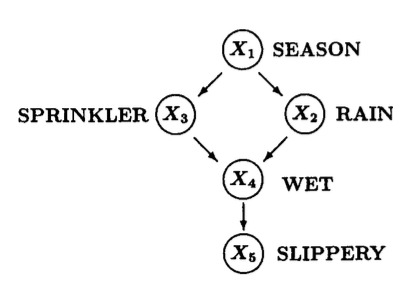
\includegraphics[width=\textwidth]{imgs/img8.png}
		\caption{Небольшая причинная байесовская сеть }
		\label{fig:scbn1}
	\end{subfigure}
%\hfill
	\begin{subfigure}[t]{0.4\textwidth}
		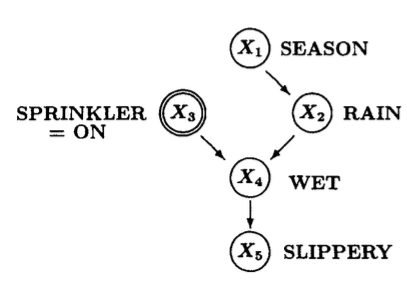
\includegraphics[width=\textwidth]{imgs/img9.png}
		\caption{После интервенции Sprinkler := On}
		\label{fig:scbn2}
	\end{subfigure}
  \label{fig:scbn}
\end{figure}

В ней все переменные бинарные (Да/Нет), кроме сезона, который понятно принимает одно из четырёх значений лето/осень/зима/весна. таким образом, для этой сети \begin{align}
	P(x) = P(x_1)P(x_2|x_1)P(x_3|x_1)P(x_4|x_2,x_3)P(x_5|x_4)
\end{align}

Допустим теперь, что мы совершаем интервенцию путём принудительного включения поливалки. Ясно, что в этом случае нам надо удалить ребро $x_1 \rightarrow x_3$, так как теперь сезон никак не может влиять на поливалку - по сути, своим \textbf{действием} мы поменяли физический закон, определяющий $x_3$. 

Тут скрывается как раз разница между наблюдением  $X_3=On$ и действием $do(X_3 = On)$: в первом случае мы просто обуславливаемся в исходной байесовской сети, во втором - в сети, которая меняется из-за интервенции. Когда мы наблюдаем, что поливалка включена, мы можем предполагать, что сейчас жаркий сезон, что наверно не было дождя и т.д. Когда мы сами включаем поливалку, понятное дело, все такие предположения становятся беспочвенными.

\define{Байесовская причинная сеть} Пусть $P(v)$ - вероятностное распределение над переменными $V$, и $P_x(v)$ - распределение, которое получается в результате интервенции $do(X=x)$. Обозначим через $P_*$ множество всех распределений с интервенциями $P_* = \{P_x(v)| X \subset V, x = instance(X)\}$. DAG G называется причинной байесовской сетью, согласованной с $P_*$ тогда и только тогда, когда $\forall P_x \in P_*$ выполняется:\\
1. $P_x(v)$ марковское относительно G\\
2. $P_x(v_i) = 1 \ \forall V_i \in X$ если $v_i$ консистентно с $X=x$ \\
3. $P_x(v_i|pa_i) = P(v_i|pa_i) \ \forall V_i \notin X$, если $pa_i$ консистентно с $X=x$

Такие ограничения на множество интервенций $P_*$ позволяют компактно представить его в виде одного графа G, и просто вычислять интервенционные распределения по правилу усечённой факторизации:
\begin{align}
	P_x(v) = \prod\limits_{\{i|V_i \notin X\}}P(v_i|pa_i) &, \ \forall v, \text{консистентного с } x
\end{align} 

Покажем, что это правило выводится из свойств байесовской причинной сети. Действительно, по свойству 1, $P_x(v) = \prod\limits_{i}P(v_i|pa_i)$.  $P_x(pa_i) = \sum\limits_{v'_i}P_x(pa_i|v'_i)P(v_i)$. Заметим далее, что если $V_i \in X$, то $P(v'_i) = \delta(v'_i = v_i)$, и потому $P_x(pa_i) = P_x(pa_i|v_i)$ в этом случае, а значит $PA_i$ независимо от $V_i$ в распределении $P_x$. Это в свою очередь значит, что $P_x(v_i | pa_i) = P_x(v_i) = 1$, что и требовалось нам показать.

Нетрудно показать верность следующих двух свойств для G - байесовской причинной сети, согласованной с $P_*(v)$

\textbf{Свойство 1}: $\forall i \ P(v_i|pa_i) = P_{pa_i}(v_i)$\\
Ну действительно, $P(v_i|pa_i) = P_{pa_i}(v_i|pa_i) = \frac{P_{pa_i}(v_i, pa_i)}{P_{pa_i}(pa_i)} = P_{pa_i}(v_i)$, где первый переход сделан по условию 3 из определения байсовской  причинной сети с $X = PA_i$, второй - так как $P_{pa_i}(v_i) = \sum\limits_{PA_i}P_{pa_i}(v_i, PA_i) = P_{pa_i}(v_i, pa_i)$, так как $P_{pa_i}$ принимает ненулевое значение только при $PA_i = pa_i$, ну и соответственно $P_{pa_i}(pa_i) = 1$.

По смыслу, это свойство означает что наблюдаемое распределение переменной $v_i$ при условии, что мы пронаблюдали $pa_i$, совпадает с распределением $v_i$, когда мы внешним вмешательством сделали $PA_i = pa_i$.

\textbf{Свойство 2}: $\forall i, \ \forall S \subset V: S \cap (\{V_i\} \cup PA_i) = \emptyset \implies \ P_{pa_i, s}(v_i) = P_{pa_i}(v_i)$\\
По условию 3 мы имеем $P_{pa_i,s}(v_i|pa_i) = P(v_i|pa_i)$.
Аналогично свойству 1, легко показать, что $P_{pa_i,s}(v_i) = P_{pa_i,s}(v_i, pa_i)$. Далее, $P_{pa_i,s}(v_i, pa_i) = P_{pa_i,s}(v_i|pa_i)P_{pa_i,s}(pa_i) = P_{pa_i,s}(v_i|pa_i)$, так как по условию 2 $P_{pa_i,s}(pa_i) = 1$. А значит, $P_{pa_i,s}(v_i) = P_{pa_i,s}(v_i|pa_i) = P(v_i|pa_i) = P_{pa_i}(v_i)$ (предпоследний переход по условию 3, последний - аналогично свойству 1).

По смыслу, это свойство описывает понятие инвариантности: как только мы контролируем $PA_i$ - все непосредственные причины $V_i$ - все прочие действия не влияют на поведение $V_i$.

Есть важное отличие между причинными связями, и вероятностным: причинные связи более "стабильны". Что это значит? По сути, причинные связи описывают механику внешнего мира, в то время как вероятностные - то, что мы знаем о мире/ во что верим. Таким образом, причинные связи не меняются при открытии нами новой информации, в этом плане они стабильны, по крайней мере до тех пор, пока физические законы (в широком смысле - законы, по которым работает окружающая среда) неизменны.

Вот пример по картинке с нашей простой байесовской причинной сетью: рассмотрим причинное отношение $S_1$ "Включение опрыскивателя не влияет на наличие дождя", и вероятностное $S_2$ "Состояние распрыскивателя независимо от наличия дождя". Согласно картинке \ref{fig:scbn1}, $S_2$ поменяется с False на True, если мы узнаем текущее время года, и обратно с True на False, если мы узнаем, мокрый асфальт, или нет. В свою очередь, узнавание любого из этих фактов не влияет на истинность $S_1$. 

\subsection*{Функциональные причинные модели}

Функциональная причинная модель состоит из набора уравнений вида 

\begin{align}
	x_i = f_i(pa_i, u_i),& \  i=1..n
	\label{eq:causal_eq}
\end{align}

Здесь $pa_i$ - множество переменных, непосредственно определяющих значение $X_i$, а $U_i$ - помехи, связанные с ненаблюдаемыми переменными.

Сравним фичи, которыми обладают функциональные модели, с фичами причинных байесовских сетей. Рассмотрим три типа запросов, от менее требовательных к детализации знаний  к более требовательным:

1. Предсказания  - будет ли покрытие мокрым, если опрыскиватель выключен?

2. Интервенции - будет ли покрытие мокрым, если мы выключим опрыскиватель?

3. Контрфакты - было бы покрытие мокрым, если бы мы выключили опрыскиватель, если мы знаем, что покрытие скользкое и опрыскиватель включён?

\subsubsection*{Предсказания}

По функциональной причинной модели построим диаграмму, проведя рёбра из $PA_i$ в $X_i$, полученный граф G называют \textbf{причинной диаграммой}.  Если G - DAG, то соответствующая модель называется \textit{полумароквской}, и значения $X$ однозначно определяются значениями $U$, $P(x)$ определяется через $P(u)$ однозначно. Если кроме того $U$ взаимонезависимы, то модель называется \textit{марковской}.

\begin{theorem}
	\textbf{Причинное марковское условие}\\
	Любая марковская причинная модель M задаёт распределение $P(x_1...x_n)$ которое удовлетворяет родительскому марковскому условию относительно диаграммы G, построенной по M. То есть, $X_i \independent Y | PA_i$ для любого $Y$ не содержащего наследников $X_i$.
	\label{th:causal_markov_condition}
\end{theorem}

Действительно, $PA_i,U_i$ однозначно определяют значение $X_i$, значит конечно $P(x_1...x_n, u_1..u_n)$ марковски совместимо с расширенным графом $G(X,U)$ (напомним, это просто значит, что распределение факторизуется согласно графу). Но тогда утверждение теоремы легко доказать, используя критерий d-разделения в расширенном графе и теорему о вероятностных следствиях d-разделения.
$\blacksquare$

Свойство марковости причинной модели можно гарантировать, если договориться о двух правилах построения модели:

1. Если $x_i$ и $x_j$ зависимы, то либо одна из них является причиной другой (не обязательно непосредственной), либо существует третья переменная, являющаяся их общей причиной (нет корреляции без причины и нет взаимной причинности).

2. Если более, чем одна переменная является следствием данной переменной $y$, то данная переменная включена в модель, т.е. $y \notin U$ - иначе бы мы наблюдали необъяснимые моделью корреляции между $x_i, x_j$, для которых $y$ - общая причина.

Второе предположение гарантирует, что $U_i \independent U_j$. Первое - то, что нет циклических зависимостей, таким образом, мы получаем марковскую причинную модель.

В чем же плюсы использования функциональных моделей по сравнению с причинными байесовскими сетями?  

Во-первых, функциональная спецификация обычно более краткая и содержит меньше параметров.

Во-вторых, в функциональных моделях проще рассуждать об условной независимости, потому что для людей естественно выводить такие предположения из предположении об отсутствии каких-то ненаблюдаемых общих причин. Человеку намного проще проверить, что все непосредственные причины события учтены, нежели проверять что переменная независима от своих ненаследников при условии известности непосредственных родителей.

Наконец, если что-то меняется в законах окружающей среды, проще учесть это в функциональном описании, нежели чисто вероятностном, так как в первом случае обычно нужно проапдейтить всего несколько уравнений.

Тем не менее, предсказание всё-таки является наиболее простой из трёх задач и решается в терминах условных вероятностей, без обязательной необходимости привлечения структурных уравнений или даже причинных байесовских сетей (обычные подойдут).

\subsubsection*{Интервенции}

Интервенции легко описывать на языке функциональных моделей. Достаточно для всех переменных, поведение которых определяется действиями, убрать соответствующие уравнения, заменив их на $x_i = c_i$. 

Кроме такого удобства, есть и другие плюсы у функциональных моделей. Во-первых, большая гибкость: если отойти от марковских моделей, мы можем описывать и циклические зависимости, таким образом, отвечая на вопросы, связанные с политиками.

Во-вторых, интервенции, меняющие параметры в уравнениях более понятны в отличие от тех, что меняют условные вероятности, так как уравнения обычно рассматриваются как описание более-менее стабильных физических процессов, в отличие от условных вероятностей. Условные же вероятности мы обычно рассматриваем как то, что выводится из общего распределения, а не как то, что его генерирует. 

Для изучения влияния интервенций обычных байесовских сетей уже недостаточно - нужны причинные байесовские сети, ну либо структурные уравнения.

\subsubsection*{Контрфакты}

Контрфактические утверждения в принципе не могут быть определены в терминах стохастических причинных моделей (стохастические это то же что байесовские сети). Рассмотрим простой пример: пусть есть модель на двух переменных $X$ - было ли дано человеку лечение или нет, и $Y$ - выжил он в итоге или нет. Допустим, что некий индивидум Джо умер после получения лекарства, и мы хотим ответить на контрфактический вопрос "Какова вероятность того, что Джо выжил \textbf{бы}, если бы ему не дали лекарство?".

Понятно, что ответить на такой вопрос по имеющимся данным невозможно: действительно, Джо умер, и никакой информации о том, что с ним было, когда он не принимал лекарство, у нас нет. Перефразирование вопроса в терминах частоты аналогичного контрфактического события в популяции не помогает в данном случае, поэтому вообще многие стат аналитики воспринимали долгое время контрфактические вопросы как метафизические, на которые невозможно ответить непосредственным тестированием.

Тем не менее, в повседневной жизни мы постоянно оперируем контрфактическими утверждениями, что является поводом считать, что такие утверждения не лишены смысла и способны нести полезную информацию / быть выводимыми из какой-то информации о мире.

Пусть в нашем примере $P(y|x) = 0.5 \ \forall x, y$. Тогда понятно, что $P(x,y) = 0.25$. Рассмотрим две функциональные модели, каждая из которых генерирует такое совместное распределение, но ведущие к различному значению искомой вероятности контрфакта Q - что субъект, умерший после лечения ($x=1, y=1$), не умер бы ($y = 0$), если бы его не лечили ($x=0$). 

Байесовская сеть, описывающая данное распределение, имеет вид, как на \ref{fig:treatment_sample_bn}

\begin{figure}[!tbph]
	\centering
	\begin{subfigure}[t]{0.3\textwidth}
		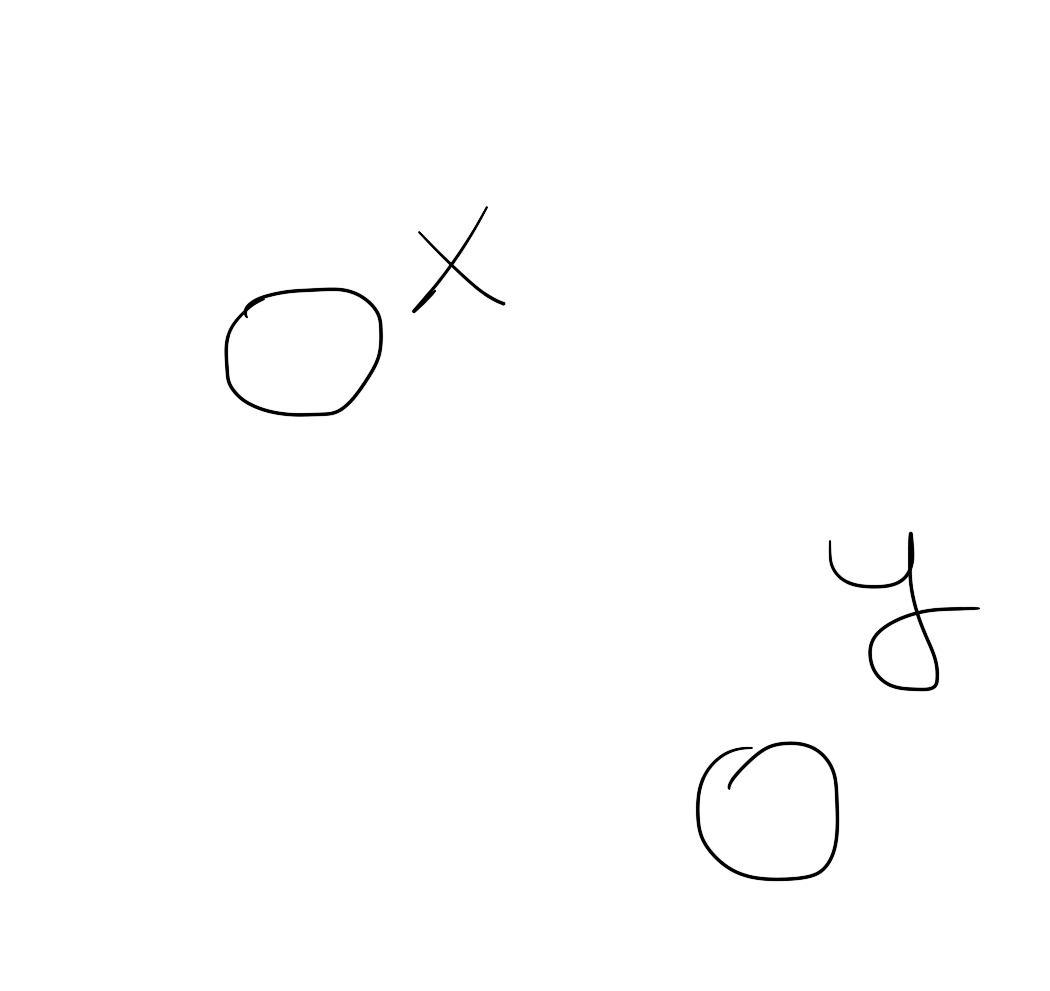
\includegraphics[width=\textwidth]{imgs/img12.png}
		\caption{Байесовская сеть для описываемого распределения}
		\label{fig:treatment_sample_bn}
	\end{subfigure}
	\begin{subfigure}[t]{0.25\textwidth}
		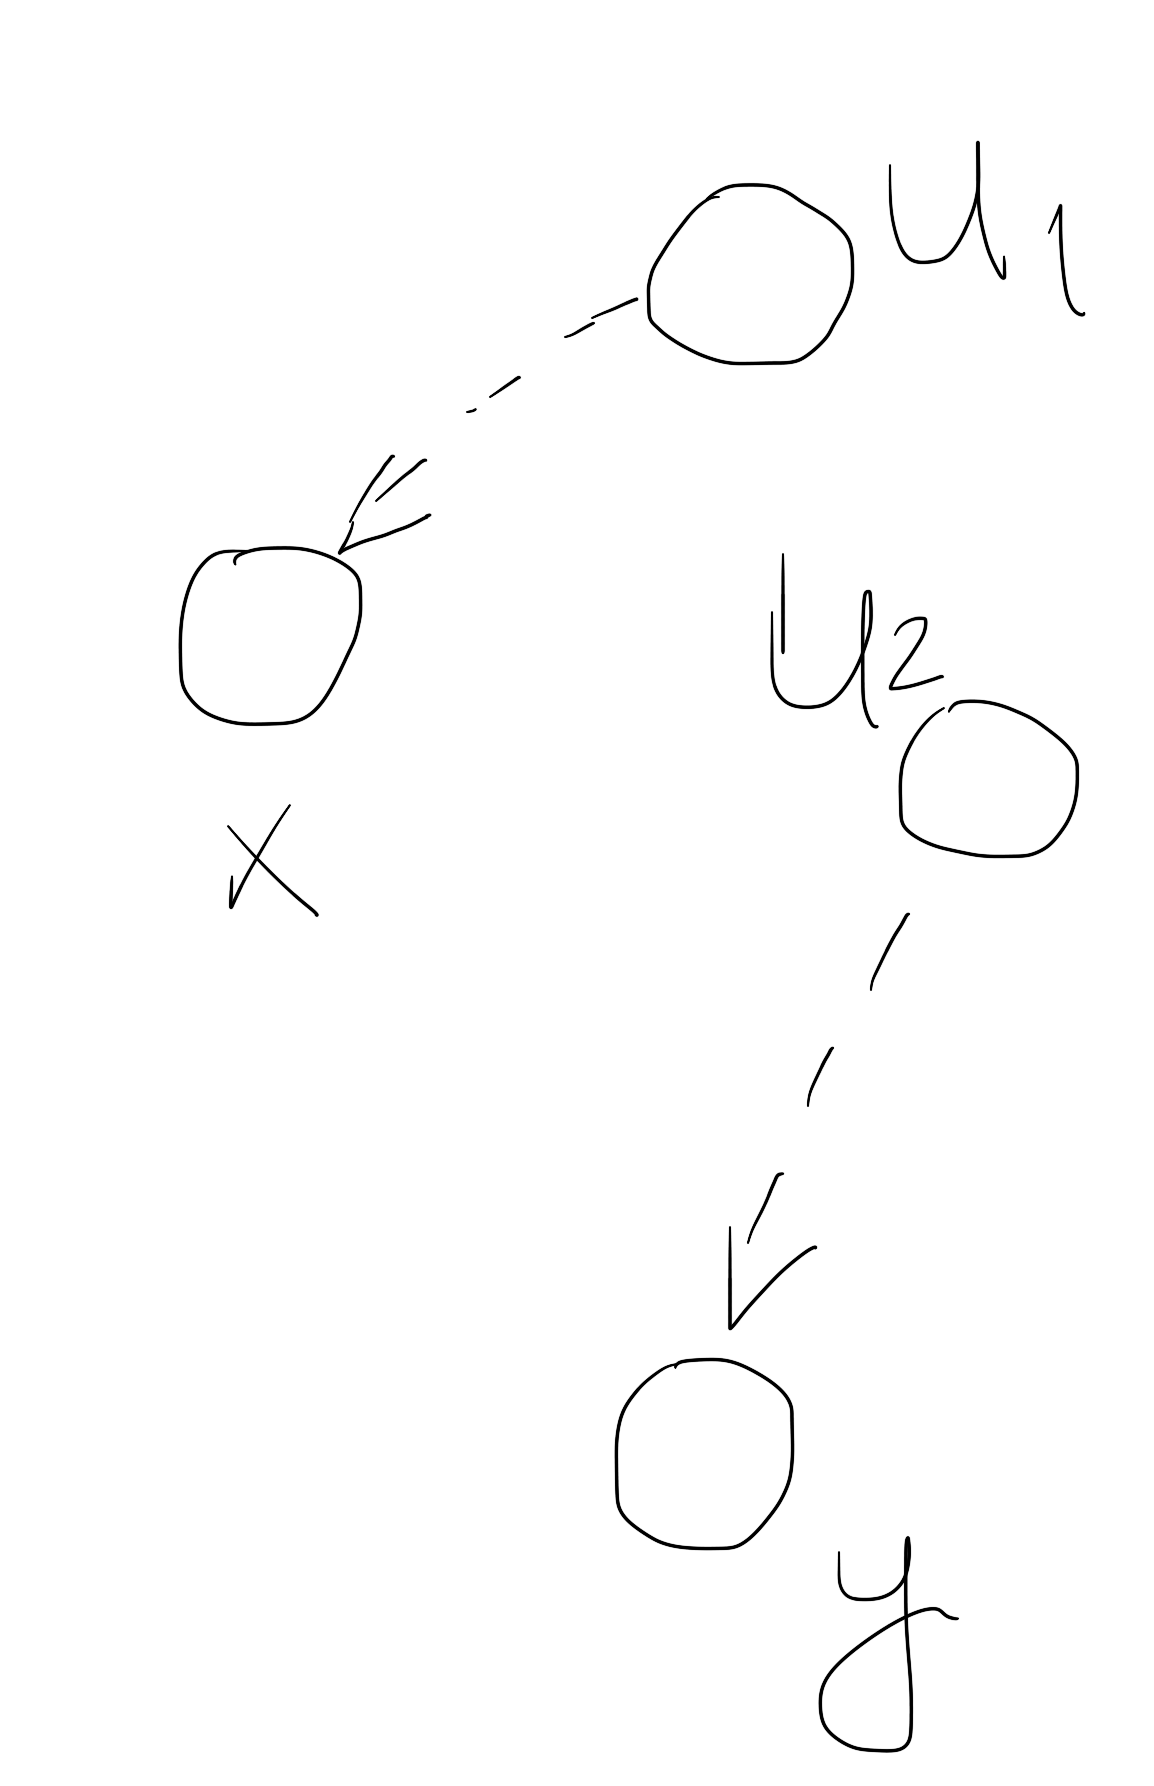
\includegraphics[width=\textwidth]{imgs/img13.png}
		\caption{Причинная диаграмма для модели 1}
		\label{fig:treatment_sample_cm1}
	\end{subfigure}
\begin{subfigure}[t]{0.25\textwidth}
	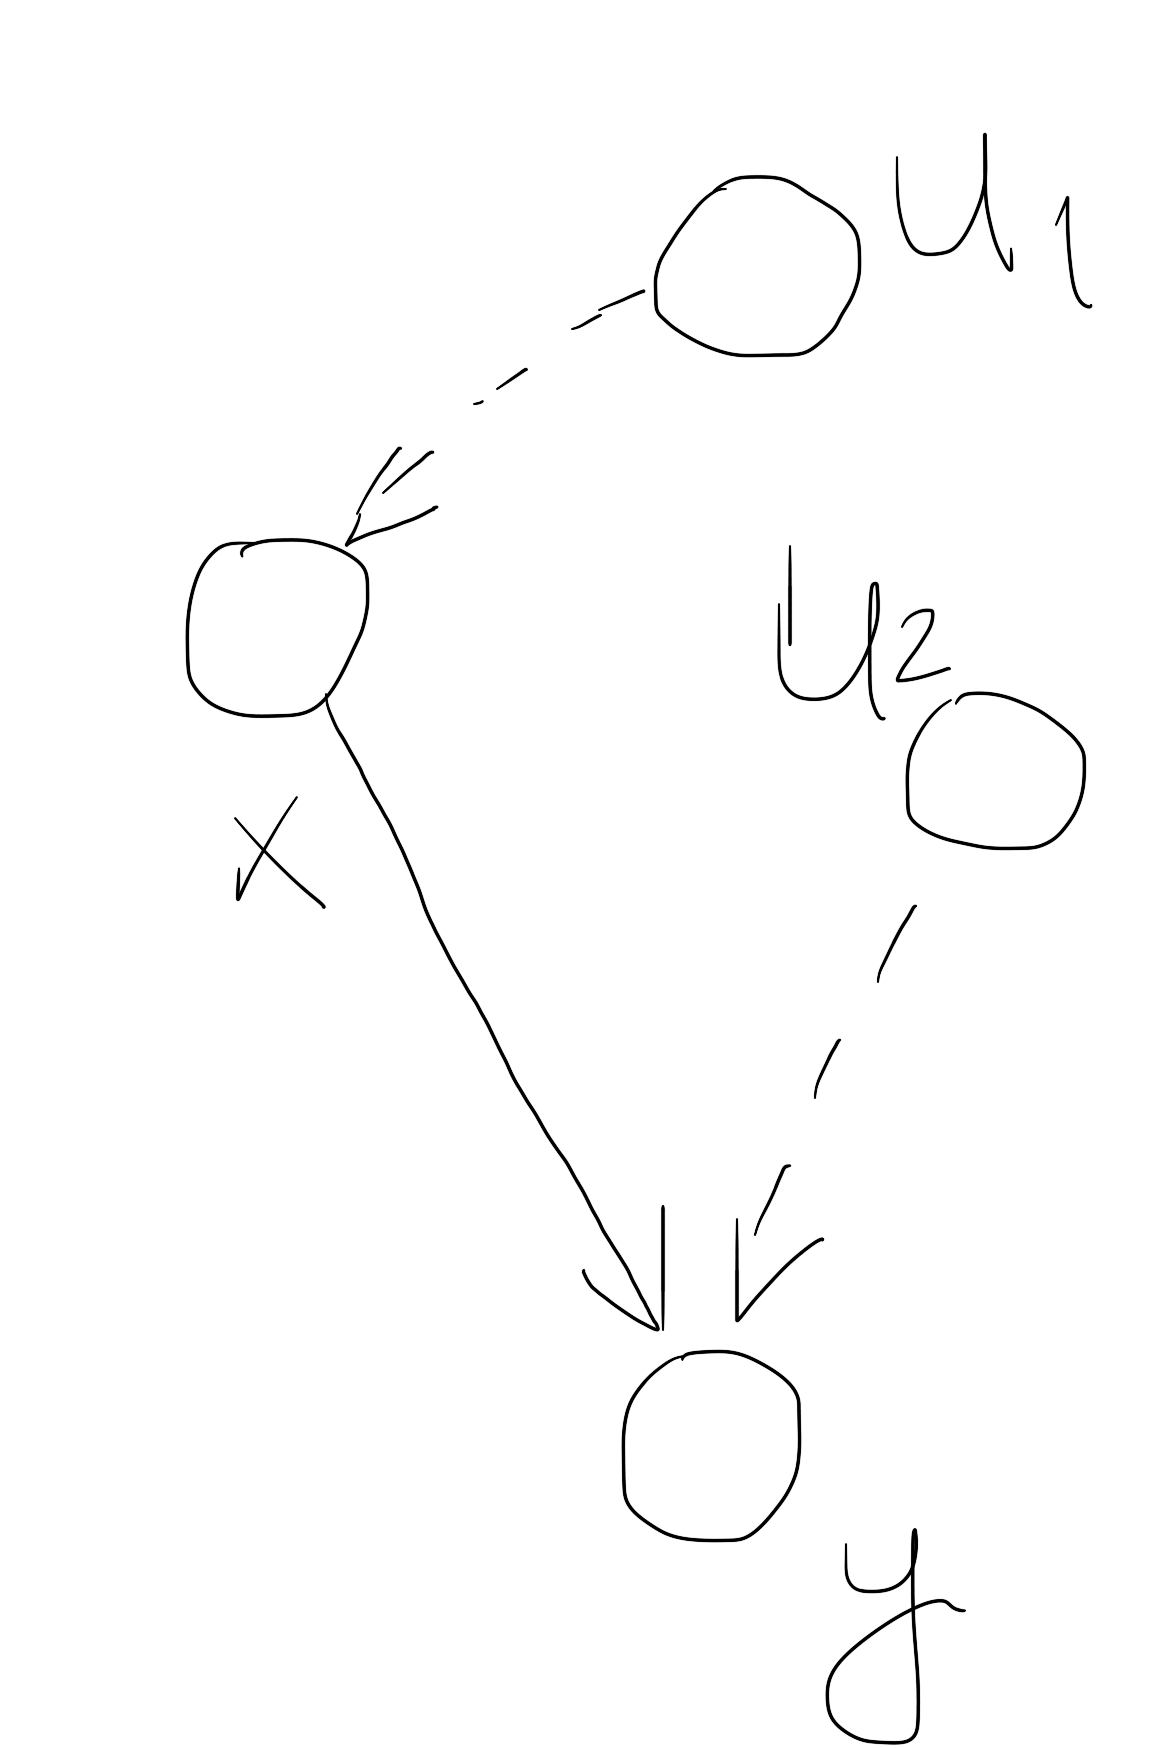
\includegraphics[width=\textwidth]{imgs/img14.png}
	\caption{Причинная диаграмма для модели 2}
	\label{fig:treatment_sample_cm2}
\end{subfigure}
\end{figure}


\textbf{Модель 1}
\begin{align}
	\begin{split}
		x = u_1\\
		y = u_2
	\end{split}
\end{align}

\textbf{Модель 2}
\begin{align}
	\begin{split}
		x &= u_1\\
		y &= u_2x + (1- x)(1- u_2)
	\end{split}
\end{align}

В первой модели, исход не зависит от лечения; во второй - исход для любого пациента зависит от лечения. Дело в том, что модель 2 описывает смесь двух подпопуляций: одной ($u_2 = 0$), в которой пациент выздоравливает только если принимает лекарство, во второй ($u_2 = 1$) пациент выздоравливает, только если лекарства ему не дают.

Эффект от лечения в этих двух моделях различен. В модели 1, $y = u_2$ и лечение не влияет на исход, так что замена $X$ c 1 на 0 для тех, кто умер и лечился, не поменяет $y = 1 = u_2$ с 1 на 0, поэтому $Q = 0$. Во второй модели, в свою очередь, замена $X$  c 1 на 0 для тех, кто умер (а это субпопуляция $u_2 = 1$), трагический исход поменяется на позитивный ($y = 1 \cdot x = 0$), то есть эффект отсутствия лечения будет $Q = 1$.

Как видим, стохастическая модель не позволяет в данном случае вычислять контрфактические вероятности: нужно знание процесса, который стоит за $P(y|x)$. С другой стороны, причинные структурные модели позволяют такие величины вычислять. Делали в данном случае мы это вычисление в три шага: сперва, мы применили имеющиеся под рукой данные $e: \{x=1, y=1\}$. Зная их, мы вывели, каковы совместимые значения $U_1, U_2$ - в данном случае только $u_1 = 1, u_2 = 1$. Вторым шагом, мы подставили $x=1$ в структурные уравнения, игнорируя уравнение для $X$ $x =u_1$.  Наконец, мы решили уравнения относительно $y$ и получили что $y \equiv 0$, то есть вероятность излечения в таком раскладе единична.

Этот подход обобщается для определения вероятности любого контрфакта $Y = y$ на данных $e$ при условии $X=x$ по структурной модели в три шага.

1. \textbf{Отведение} - заменяем $P(u) \leadsto P(u|e)$

2. \textbf{Действие} - заменяем уравнения, определяющие $X$, на  $X=x$

3. \textbf{Предсказание} - используем модифицированную модель для вычисления вероятности $Y = y$.

Если перекладывать этот метод на временные метафоры, то первый шаг - это объяснение прошлого с учётом имеющихся доказательств/данных; второй шаг - минимальное изменение курса истории чтобы согласовать мир с $X = x$; третий шаг - это предсказание будущего $Y$ при условии нашего нового понимания прошлого и нашего альтернативного настоящего.

В целом, это самая сложная из трёх задач, и она уже в свою очередь не решается без привлечения механизма структурных уравнений.

\subsection*{Причинная и статистическая терминология}

\define{Вероятностный параметр} - любая величина, определяемая через совместное распределение переменных.

\define{Статистический параметр} - любая величина. определяемая через совместное распределение наблюдаемых переменных, без каких либо предположений о существовании/несуществовании ненаблюдаемых переменных. Примерами являются условное матожидание $E(Y|x)$, коэффициент регрессии $r_{XY}$, значение плотности вероятности в $x = 0, y = 1$.

\define{Причинный параметр} - любая величина, определяемая через причинную модель (которая задана в виде структурных уравнений) как в 
\ref{eq:causal_eq} и не являющаяся в то же время статистическим параметром. Примерами является параметр функции $f_i(pa_i, u_i)$, имеет ли $X_9$ влияние на $X_3$ при некотором $u$, ожидаемое значение $Y$ при совершении интервенции $do(X=0)$.

\define{Статистическое предположение} - предположение о совместном распределении наблюдаемых переменных: например, что оно марково относительно некоторого DAG, или является многомерным нормальным.

 \define{Причинное предположение} - любое ограничение на причинную модель, которое не представимо статистическими предположениями. Например, что $f_i$ линейно, или что $x_3 \notin pa_4$. Причинные предположения могут как иметь статистические следствия, так и нет. В первом случае говорят, что причинное предположение "проверяемо" или "фальсифицируемо". Часто, хоть и не всегда, причинные предположения фальсифицируемы через эксперимент, в этом случае говорят об "экспериментальной фальсифицируемости". Например, предположение, что $X$ не имеет эффекта на $E[Y]$ в рассмотренной ранее модели два фальсифицируемо экспериментом, в то время как предположение "$X$ может вылечить определенного субъекта популяции" - нет. 
 
 \subsection*{Два ментальных барьера к причинному анализу}

Есть две сложности, с которыми мы сталкиваемся: во-первых, за каждым причинным высказыванием стоят причинные предположения, которые не выводятся из совместного распределения, и соответственно, они не проверяемы с помощью одних лишь наблюдаемых данных. Эти предположения предоставляются людьми, то есть приходится полагаться на какое-то экспертное мнение.

Во-вторых, для математического описания причинной теории нужна новая нотация: как мы выяснили, чисто вероятностного языка недостаточно. Например, на языке теории вероятностей (то есть через функции распределения) невозможно выразить причинную связь симптома и болезни: мы можем только описать их зависимость через $P(disease | symptom)$, но мы не можем отличить, причинная эта зависимость или статистическая.

\section{Теория вывода причинности}

\subsection*{Интуиция}
Начнем с интуиции, которая стоит за причинно-следственными связями. Обычно необходимым условием является временная зависимость - причина происходит до следствия. Однако, очевидно, это далеко не всегда является достаточным условием для наличия причинной связи, поэтому остается вопрос, же ее установить?

Возможно ли в целом какое-то выявление причинно-следственных связей? На самом деле, да. Рассмотрим пример, где есть три события $A, B, C$ и мы знаем, что $A$ зависимо с $B$, $B$ зависимо с $C$, но $A$ и $C$ независимы. В таком случае, если немного подумать, выходит, что наиболее простой граф, описывающий такую конфигурацию, выглядит как на \ref{fig:abc}


\begin{figure}[h]
	\begin{center}
	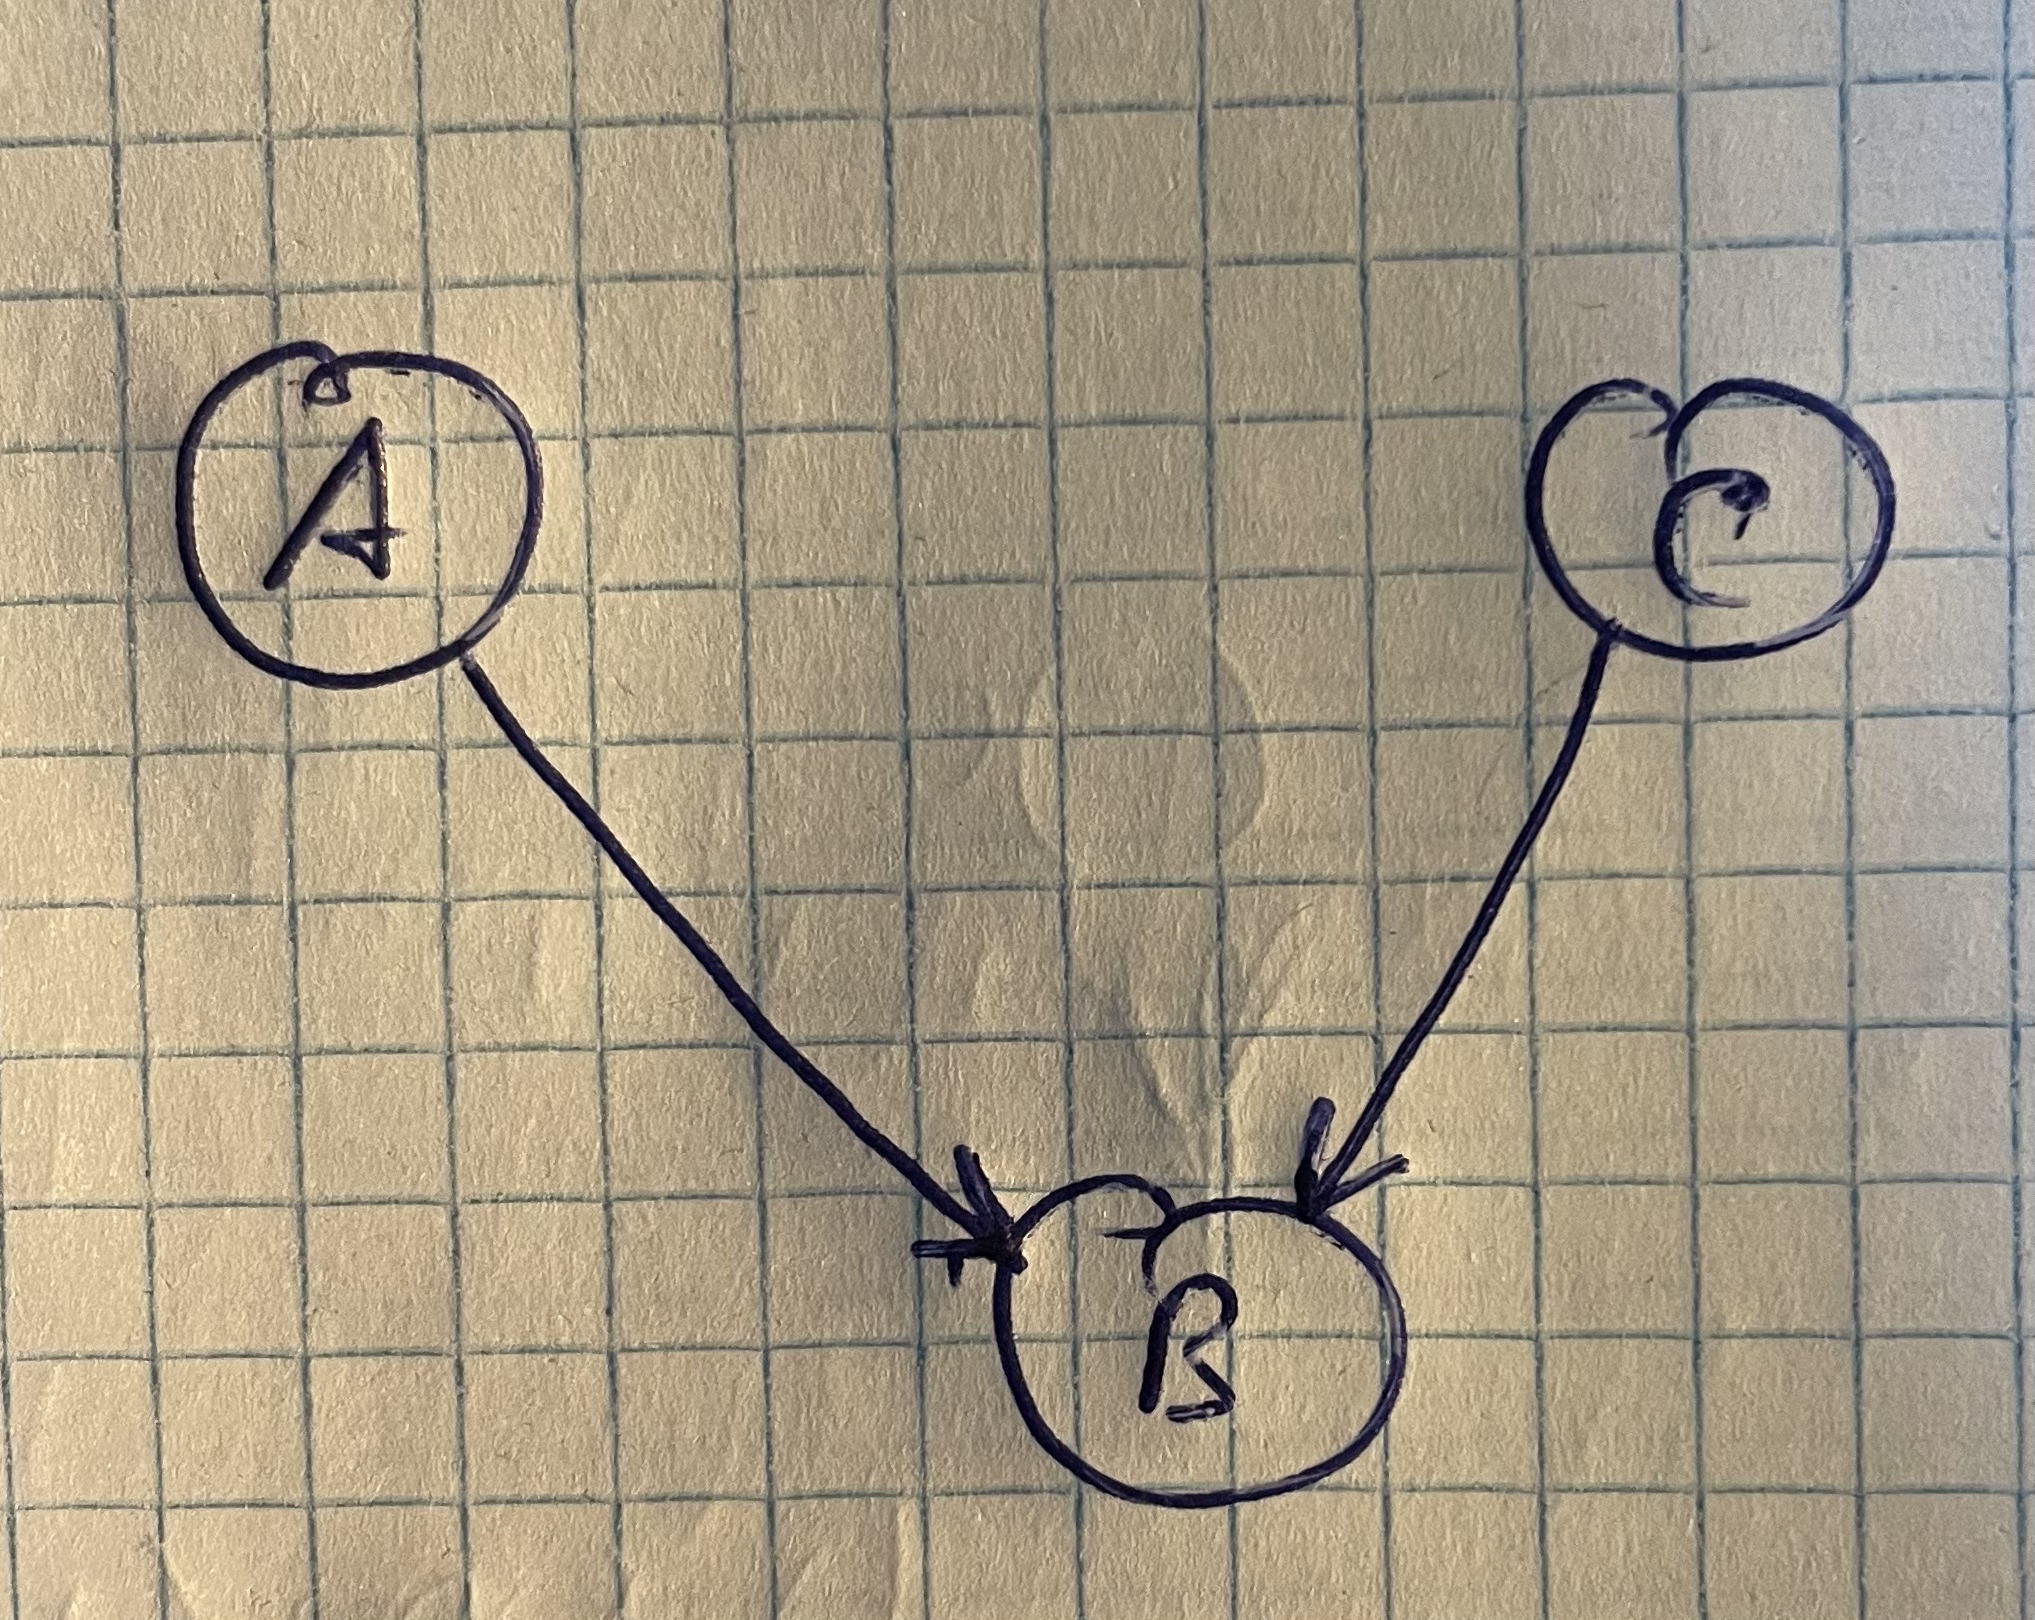
\includegraphics[scale=0.1]{imgs/img1.png}
	\end{center}
	\caption{A, C безусловно независимы, но зависимы при наблюдаемом следствии B}
	\label{fig:abc}
\end{figure}

\subsection*{Фреймворк}

Будем рассматривать задачу определения причинно-следственных связей в виде индукционной игры (индукционность в смысле что про некоторым примерам выводится какое-то общее правило), в которую ученый играет с природой (красивая формулировка конечно XD). предполагается, что у природы есть стабильные причинно-следственные механизмы, которые можно определить функциональными зависимостями между переменными, некоторые из которых впрочем ненаблюдаемы.

\define{Причинная структура (causal structure)} множества переменных $V$ - это DAG, в котором вершинам соответствуют переменные, а рёбрам - прямая функциональная зависимость между соответствующими переменными.

Причинная структура - это грубо говоря макет для \textbf{причинной модели} - точного определения того, как одни переменные влияют на другие.

\define{Причинная модель (causal model)}  - пара $(D, \Theta_D)$ из причинной структуры $D$ и множества параметров $\Theta_D$, ей соответствующих, то есть описывающих конкретные функциональные зависимости между переменными $V$ в виде $x_i = f_i(pa_i, u_i)$ $\forall x_i \in V$, где $PA_i$ - родители $x_i$ согласно $D$, $U_i$ - случайный шум, вероятностное распределение над которым также определяется $\Theta_D$, $U_i \independent U_j$.

Шум, влияющий на значение переменных, можно рассматривать например как следствие ненаблюдаемости некоторых переменных. Такая модель, согласно данному ранее определению, является марковской, а потому по теореме \ref{th:causal_markov_condition} задаёт распределение, марковски согласованное с $D$.

Теперь задачу, поставленную перед гипотетическим учёным, можно сформулировать в виде восстановления причинной структуры, а затем и модели, при условии что он наблюдает лишь значения некоторого подмножества переменных $O \subset V$.

\subsection*{Выбор модели (бритва Оккама)}

Вообще говоря, так как $V$ неизвестно, можно придумать сколь угодно много разных моделей, которые смогу зафитить данное (эмпирически определённое) распределение $P(O)$, путём различного введение скрытых переменных. Например, можно ввести одну скрытую переменную $U$, которая будет причиной всех наблюдаемых переменных $O$, при этом никаких причинно-следственных связей между наблюдамемыми переменными в такой модели не будет, причинная структура для такой модели представлена на \ref{fig:useless_model}.

\begin{figure}[h]
	\begin{center}
		\includegraphics[scale=0.1]{imgs/img2.png}
	\end{center}
	\caption{Довольно бесполезная причинная структура}
	\label{fig:useless_model}
\end{figure}

С другой стороны, считая $V=O$, но не имея никаких временных подсказок, учёный не может отбросить возможность того, что подлежащая структура - это полный DAG, где все вершины связаны со всеми в произвольном порядке - такая структура может имитировать поведение любой структуры. 

Идея выбора модели состоит в том, чтобы в некотором смысле она была наиболее простой/минимальной относительно тех данных, которые наблюдаемы.

Дальше введем не совсем формальное пока-что определение выведенной причинности (пока полагаем, что все переменные наблюдаемые)

\define{Выведенная причинность (предв.)} Переменная $X$ имеет причинное влияние на переменную $Y$, если существует направленный путь из $X$ в $Y$ в любой минимальной \textbf{причинной} структуре, согласованной с данными.

\define{Скрытая структура (latent structure)} это пара $L = (D, O)$, где $D$ - причинная структура над $V$, $O \subset V$ - множество наблюдаемых переменных.

\define{Предпочтение структуры (structure preference)} структура $L = (D, O)$ предпочтительнее структуры $L' = (D', O')$ (пишут $L \preceq L'$) если $D'$ эквивалентно $D$ на множестве наблюдаемых переменных $O$, т.е. тогда и только тогда, когда  $\forall \Theta_D \  \exists \Theta_{D'} : P_{[O]}((D', \Theta_{D'})) = P_{[O]}((D, \Theta_{D}))$. 

Латентные структуры называются эквивалентными, если $L \preceq L'$ и $L' \preceq L$. 

\define{Минимальность (minimality)} структуры $L$ относительно класса структур $C$ означает её предпочтительность относительно всех других структур этого класса: $\forall L' \in C \ L \preceq L'$.

\define{Согласованность} латентной структуры $L = (D, O)$ с распределением $\hat P$ над $O$ означает возможность разместить $\hat P$ в данной латентной структуре, то есть что $\exists \Theta_D : P((O, \Theta_D)) = \hat P$.


\define{Выведенная причинность} С данной $\hat P$ над $O$, переменная $X$ имеет причинное влияние на переменную $Y$, если существует направленный путь из $X$ в $Y$ в любой минимальной \textbf{латентной} структуре.

Надо отметить, что экспрессивная мощность латентной структуры тем выше, чем меньше в ней закодировано независимостей между переменными: таким образом, структуры с меньшим числом независимостей, согласованные с данными, будут менее предпочтительны, чем структуры с большим числом независимостей в причинной структуре.

\subsection*{Стабильные распределения}

Концепция минимальности латентной структуры позволяет корректно и непротиворечиво получать выводы о причинных связях переменных. Однако, это не всегда вычислительно просто - различных конфигураций структур может быть очень много, и проверять каждую из них на минимальность может быть очень дорого. К тому же, вообще говоря, может же оказаться, что настоящий процесс, генерировавший данные, все таки был порожден моделью, отличной от минимальной? Чтобы упростить себе жизнь, предлагается ввести в рассмотрение ещё один принцип, помимо минимальности - принцип \textit{стабильности}. 

Начнем с небольшого примера. Рассмотрим процесс, в котором есть две честные монетки. Множеством событий будет выпадение монетки $A$, выпадение монетки $B$, и событие $C$ - "монетки выпали одинаковой стороной". нетрудно заметить, что любая пара переменных безусловно независима, но зависима при условии третьей переменной (например, $P(A=1) = P(A=1|B) = 0.5\ \forall B$, но $P(A=1|B=1) =0.5\neq P(A=1|C=1,B=1) = 1$). Таким образом, любая из структур на \ref{fig:choice} допустима с точки зрения данных и является минимальной. В то же время, если чуть пошатать параметры распределения, например сделать $P(A=1) = 0.6, P(A=0)=0.4$, то уже однозначно не подойдет структура, где $C$ и $B$ независимы безусловно, так как будет $P(C=1) = 0.5$, но $P(C=1|B=1) = 0.6$. Аналогично можно пошатать вероятности для второй монетки, сделав её не совсем честной, и отбросить модель, где $A$ и $C$ независимы.

\begin{figure}[h]
	\begin{center}
		\includegraphics[scale=0.07]{imgs/img3.png}
	\end{center}
	\caption{Какую из трех причинных структур выбрать?}
	\label{fig:choice}
\end{figure}

Для того, чтобы разрулить такие неоднозначности, вводится понятие стабильности:

\define{Стабильность (распределения)} Пусть $I(P)$ - множество всех независимых отношений переменных, заданных через $P$. Причинная модель $M = (D, \Theta_D)$ генерирует стабильное распределение тогда и только тогда когда в $P((D, \Theta_D))$ нет никаких лишних независимостей, т.е. $I(P((D, \Theta_D))) \subset I(P(D, \Theta_{D'}))\ \forall \Theta_{D'}$.

По смыслу, при варьировании параметров от $\Theta$ к $\Theta'$ никакие независимости не должны рушиться, если распределение стабильно. Что пока непонятно - а как выбирать, какие из вероятностей шатать: видимо те которые не ноль? Тогда и правда из стабильности остается только один вариант из трех в приведенном выше примере.

Стабильность означает, что распределение $P$ имеет \textbf{идеальное} представление в виде DAG, то есть граф не просто I-map, но и D-map, и соответственно изоморфен распределению. 

\subsection*{Реконструкция причинной структуры (DAG)}

Когда все переменные наблюдаемы, если использовать принципы минимальности и стабильности, мы всегда будем получать единственную (с точностью до эквивалентности) причинную структуру (эквивалентные структуры - которые шарят одни и те же независимости, то есть один и тот же скелет и v-структуры).

Так как у подлежащей структуры мб эквивалентные, полученный DAG не будет однозначно определяться, поэтому лучшее, что можно сделать - определить его класс эквивалентности. Такой класс эквивалентности называют \textbf{шаблоном} (\textbf{pattern}), и он представляет из себя частично ориентированный граф (ориентируются только те рёбра, которые одинаково направлены во всех графах данного класса эквивалентности).

\textbf{IC (Inductive Causation) Algorithm}

\textbf{Вход:} $\hat P$ - стабильное распределение над переменными $V$.

\textbf{Выход:} $H(\hat P)$ - шаблон, согласованный с $\hat P$.

\textbf{Шаг 1:} Строится неоринетированный граф $D$ на вершинах $V$. Ребром соединяются любые две вершины $a, b$ такие, что $\not\exists S_{ab} \subset V \backslash \{a,b\}:\ a \independent b | S_{ab}$ 

\textbf{Шаг 2:}  $\forall a, b \in V: (a,c) \not \in E$ перебираются их общие соседи $c: (a,c)\in E,  (b,c) \in E$ и проверяется, $c \in S_{ab}$ или нет: если нет, рёбра $a,c$ и $b,c$ ориентируются в сторону $c$ (то есть создаёется новая $v-$структура).

\textbf{Шаг 3:} Ориентируем оставшиеся рёбра, если это можно сделать однозначно при условии, что надо соблюсти условия \begin{itemize}
	\item ацикличности
	\item не добавления новых $v-$структур
\end{itemize}

Первый шаг отвечает за то, чтобы построить скелет графа - действительно, следует соединять только те вершины, которые не разделимы никаким множеством других вершин. Второй - за то, чтобы ориентировать все обязательные v-структуры - потому что раз $c \notin S_{ab}$, то $a - c - b$ должен быть заблокирован без обуславливания на $c$, а значит, $a \rightarrow c \leftarrow b$. Ну а третий шаг просто итеративно добавляет ориентации тем рёбрам, про которые можно однозначно вывести их направление после всех предыдущих манипуляций. При этом, на третьем шаге мы не добавляем новые v-структуры, так как все необходимые добавлены на шаге 2.

\subsection*{Реконструкция латентной структуры}

Когда природа решает "спрятать" некоторое подмножество переменных, наблюдаемое распределение $\hat P$ может уже оказать нестабильным относительно наблюдаемого множества переменных $O \subset V$.

\define{Проекция латентной структуры} $L_{[O]} = (D_{[O]}, O)$ для структуры L это  латентная структура со следующими свойствами:
 
1. Любая ненаблюдаемая переменная в $D_{[O]}$ является общей причиной \textit{ровно двух} наблюдаемых переменных

2. Для любого стабильного распределения $P$, генерируемого $L$, существует распределение $P'$, генерируемое $L_{[O]}$, имеющее те же независимости, что и $P$: $I(P_{[O]}) = I(P'_{[O]})$. 

\begin{theorem}
	У любой латентной структуры существует как минимум одна проекция.
\end{theorem}

Оставим пока это утверждение без доказательства.
$\blacksquare$

Проекции удобно представлять в виде двунаправленного графа, в котором вершины соответствуют только наблюдаемым переменным. Любое двунаправленное ребро в графе означает существование общей скрытой причины двух наблюдаемых переменных.

Можно показать, что имея проекцию произвольной минимальной латентной структуры, генерирующей $\hat P$, можно разметить рёбра проекции так, что по этой разметке можно проверять наличие причинного пути в любой минимальной модели для $\hat P$. Для построения проекции с последующей разметкой рёбер существует алгоритм $IC^*$, разбивающий рёбра на 4 типа:

1. Помеченная стрелка $ a \xrightarrow{*} b$ - означает наличие направленного ребра из $a$ в $b$ в подлежащей модели.

2. Непомеченная стрелка $a \rightarrow b$ - означает либо наличие направленного ребра в подлежащей модели, либо существование общей скрытой причины $a \leftarrow L \rightarrow b$.

3. Непомеченная двунаправленная стрелка $a \leftrightarrow b$ означает наличие общей скрытой причины в подлежащей модели $a \leftarrow L \rightarrow b$

4. Неориентированное ребро $a - b$ означает что в подлежащей модели есть либо ребро  $a \rightarrow b$, либо $a \leftarrow b$, либо общая причина $a \leftarrow L \rightarrow b$

\textbf{IC$^*$ (Inductive Causation with Latent Variables) Algorithm}

\textbf{Вход:} $\hat P$ - распределение над переменными $O$, стабильное относительно некоторой латентной структуры.

\textbf{Выход:} $core(\hat P)$ - размеченный шаблон, согласованный с $\hat P$.

\textbf{Шаг 1:} Строится неориентированный граф $D$ на вершинах $O$. Ребром соединяются любые две вершины $a, b$ такие, что $\not\exists S_{ab} \subset V \backslash \{a,b\}:\ a \independent b | S_{ab}$ 

\textbf{Шаг 2:} Для любых двух не соединенных ребром вершин $a, b$ с общим соседом $c$, проверяется, $c \in S_{ab}$. Если нет, то стрелки направляются в сторону $c$, образуя v-структуру: $a \rightarrow c \leftarrow b$, иначе ничего не делается.

\textbf{Шаг 3:} В полученном частично ориентированном графе, ориентируем все возможные концы рёбер, итеративно добавляя стрелки рёбрам по двум правилам:

1. Для любой пары $a, b$ не соединенных ребром вершин, если $a \rightarrow c$ и нет стрелки из $b \rightarrow c$, то добавить стрелку $c \xrightarrow{*} b$

2. Если $a,b$ смежны и существует направленный путь $a \xrightarrow{*} ... \xrightarrow{*} b$ состоящий из только из помеченных стрелок, то добавить $a \rightarrow b$. 

\subsection*{Локальный критерий для вывода причинных связей}

\define{Потенциальная причина} переменная $X$ является потенциальной причиной $Y$, если выполняются следующие условия:

1. $\not \exists S: X \independent Y | S$, то есть $X,Y$ зависимы в любом контексте. Под контекстом понимается набор переменных с конкретными значениями.

2. Существует контекст $S$ и переменная $Z$: 

- $X \independent Z | S$

- $Y \not \independent Z | S$

Для лучшего понимания можно обратиться к рисунку \ref{fig:x_potential_cause_of_y}: ясно, что $Y$ \textit{не может} быть причиной $X$, иначе будет существовать незаблокированный $S$ путь $Z \leadsto Y \rightarrow X$, а потому либо $X$ - истинная причина $Y$, либо они случайно ассоциированны из-за того, что существует общая ненаблюдаемая причина для них. 

\begin{figure}[h]
	\begin{center}
		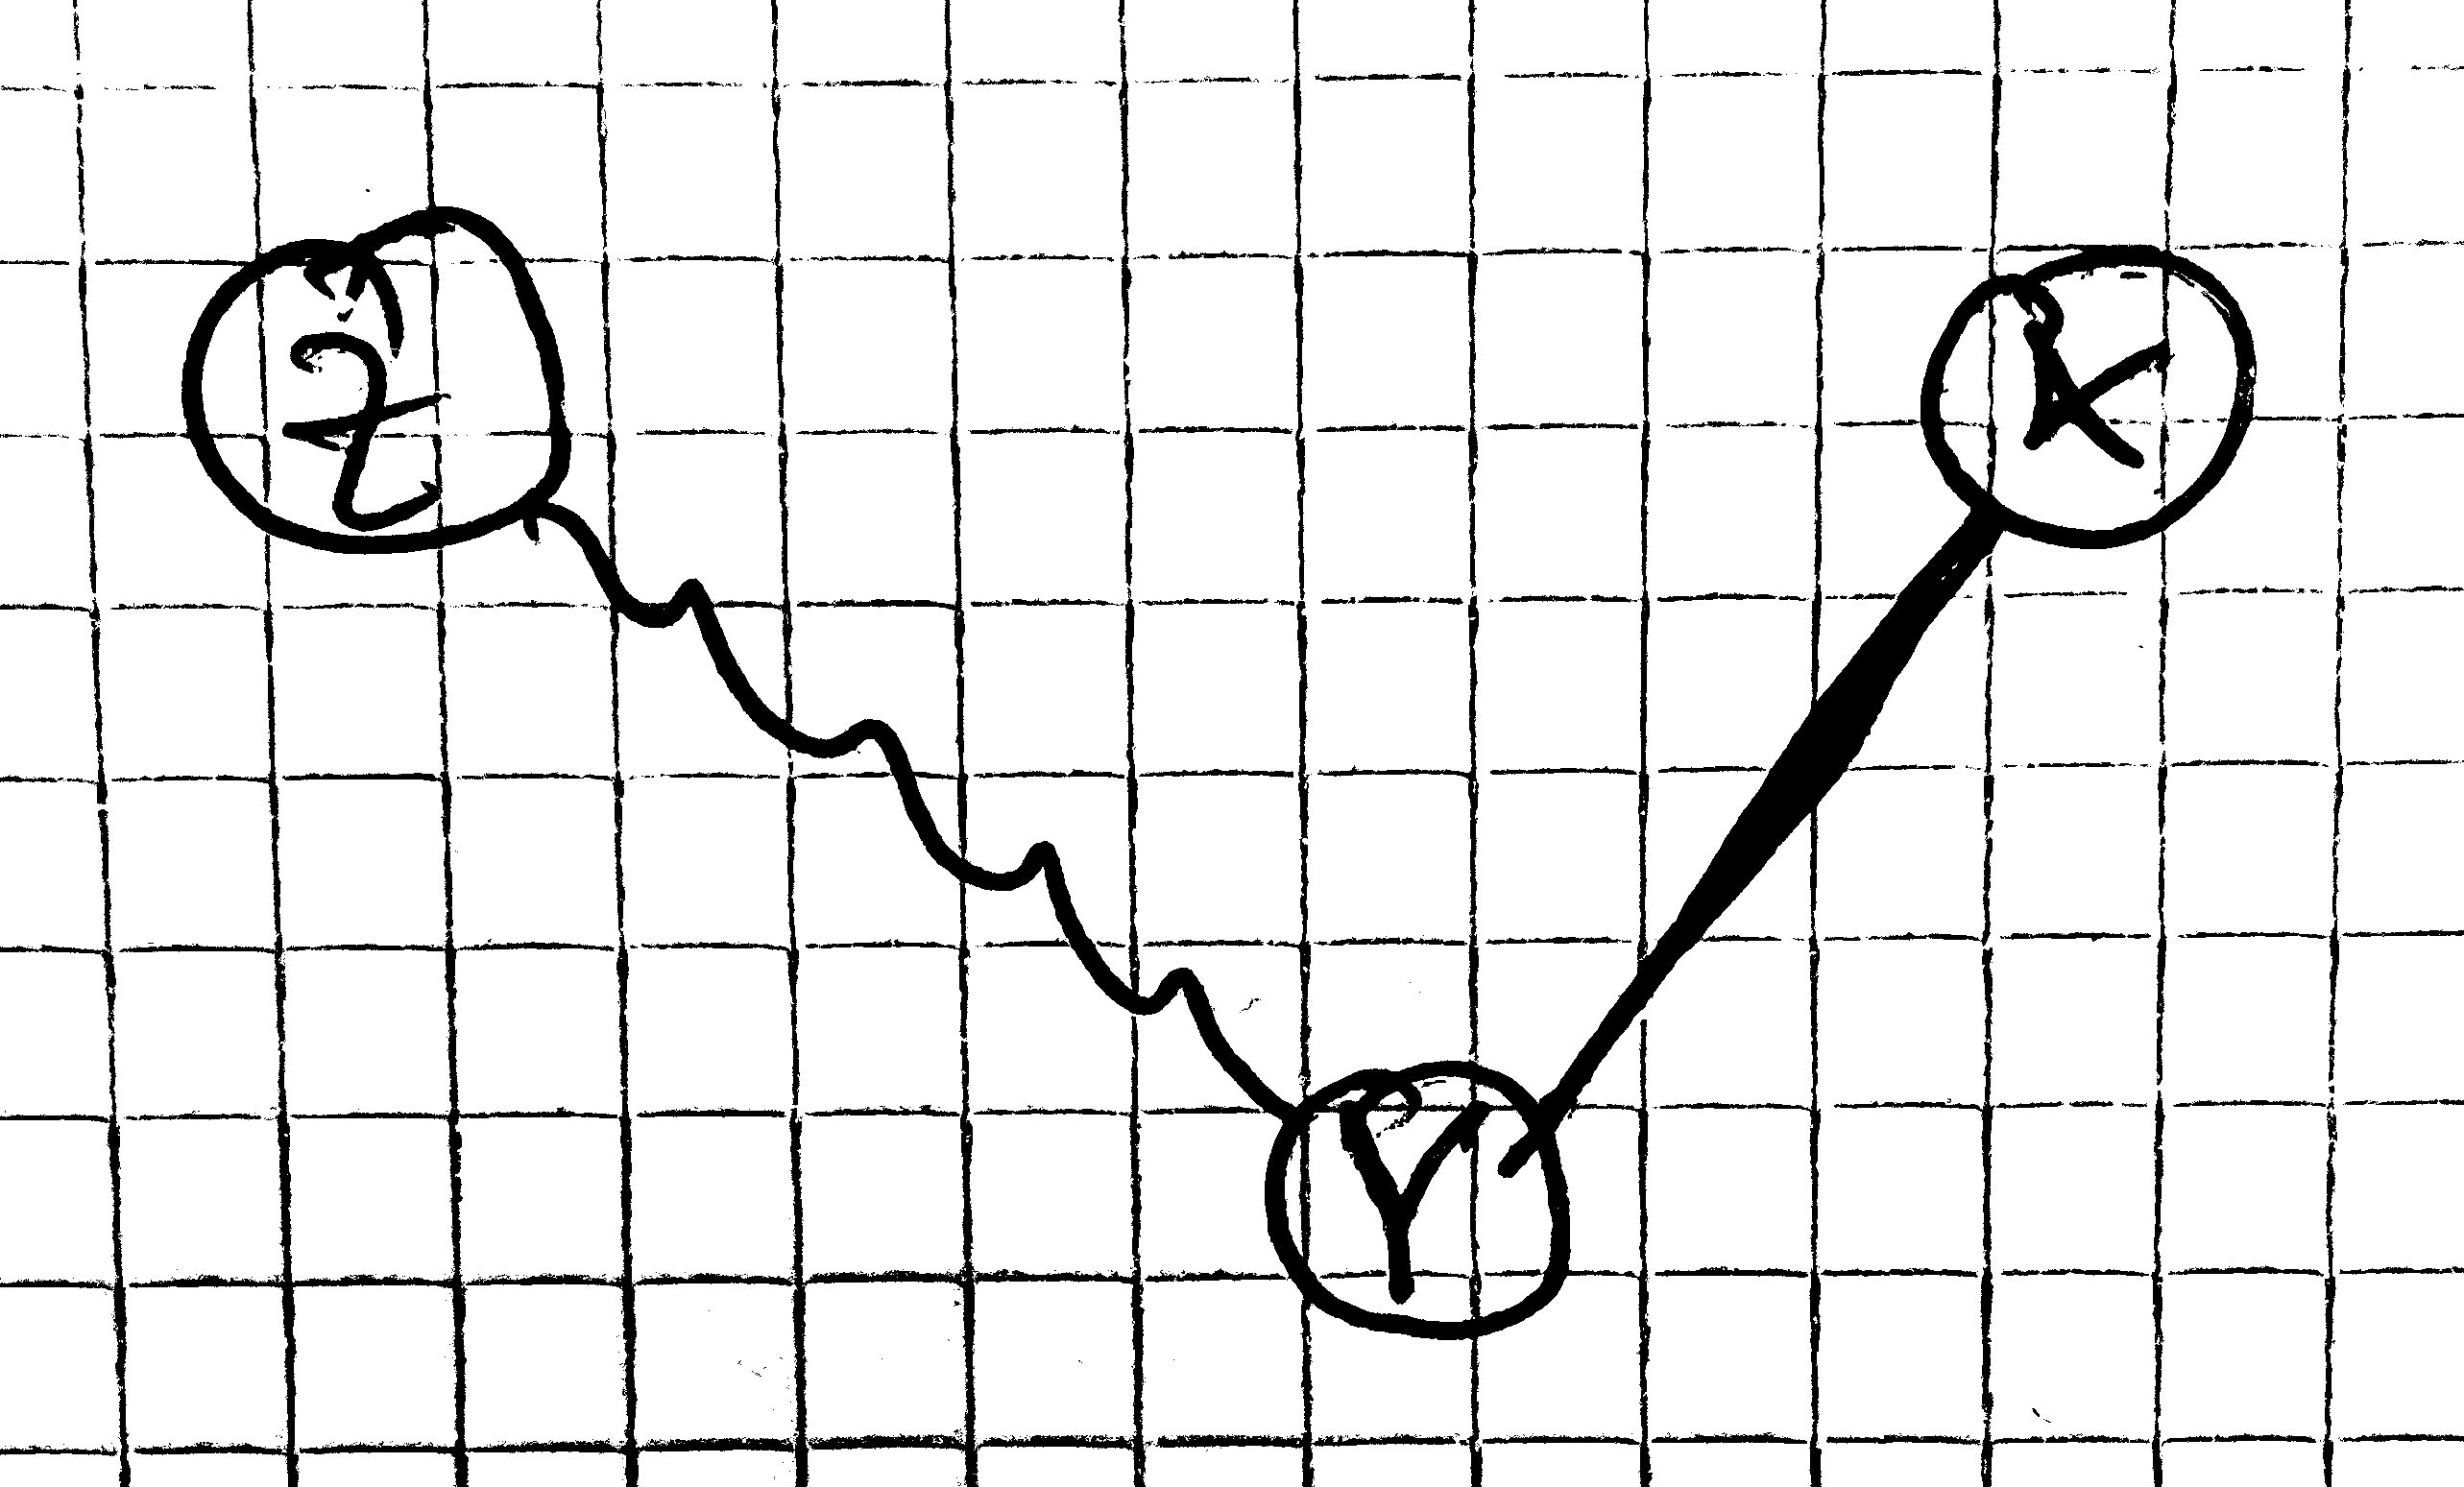
\includegraphics[scale=0.07]{imgs/img17.png}
	\end{center}
	\caption{X - потенциальная причина Y, Y - точно не может быть причиной X}
	\label{fig:x_potential_cause_of_y}
\end{figure}


\define{Подлинная причина} Переменная $X$ имеет подлинное причинное влияние на переменную $Y$ если существует переменная $Z$, такая, что выполняется одно из двух условий:

1. $X, Y$ зависимы в любом контексте, и существует контекст $S$:

* $Z$ - потенциальная причина $X$ в смысле предыдущего определения

* $Z \not \independent Y | S$

* $Z \independent Y | S \cup X$

2. $X, Y$ находятся в транзитивном замыкании первого пункта. 

\begin{figure}[h]
	\begin{center}
		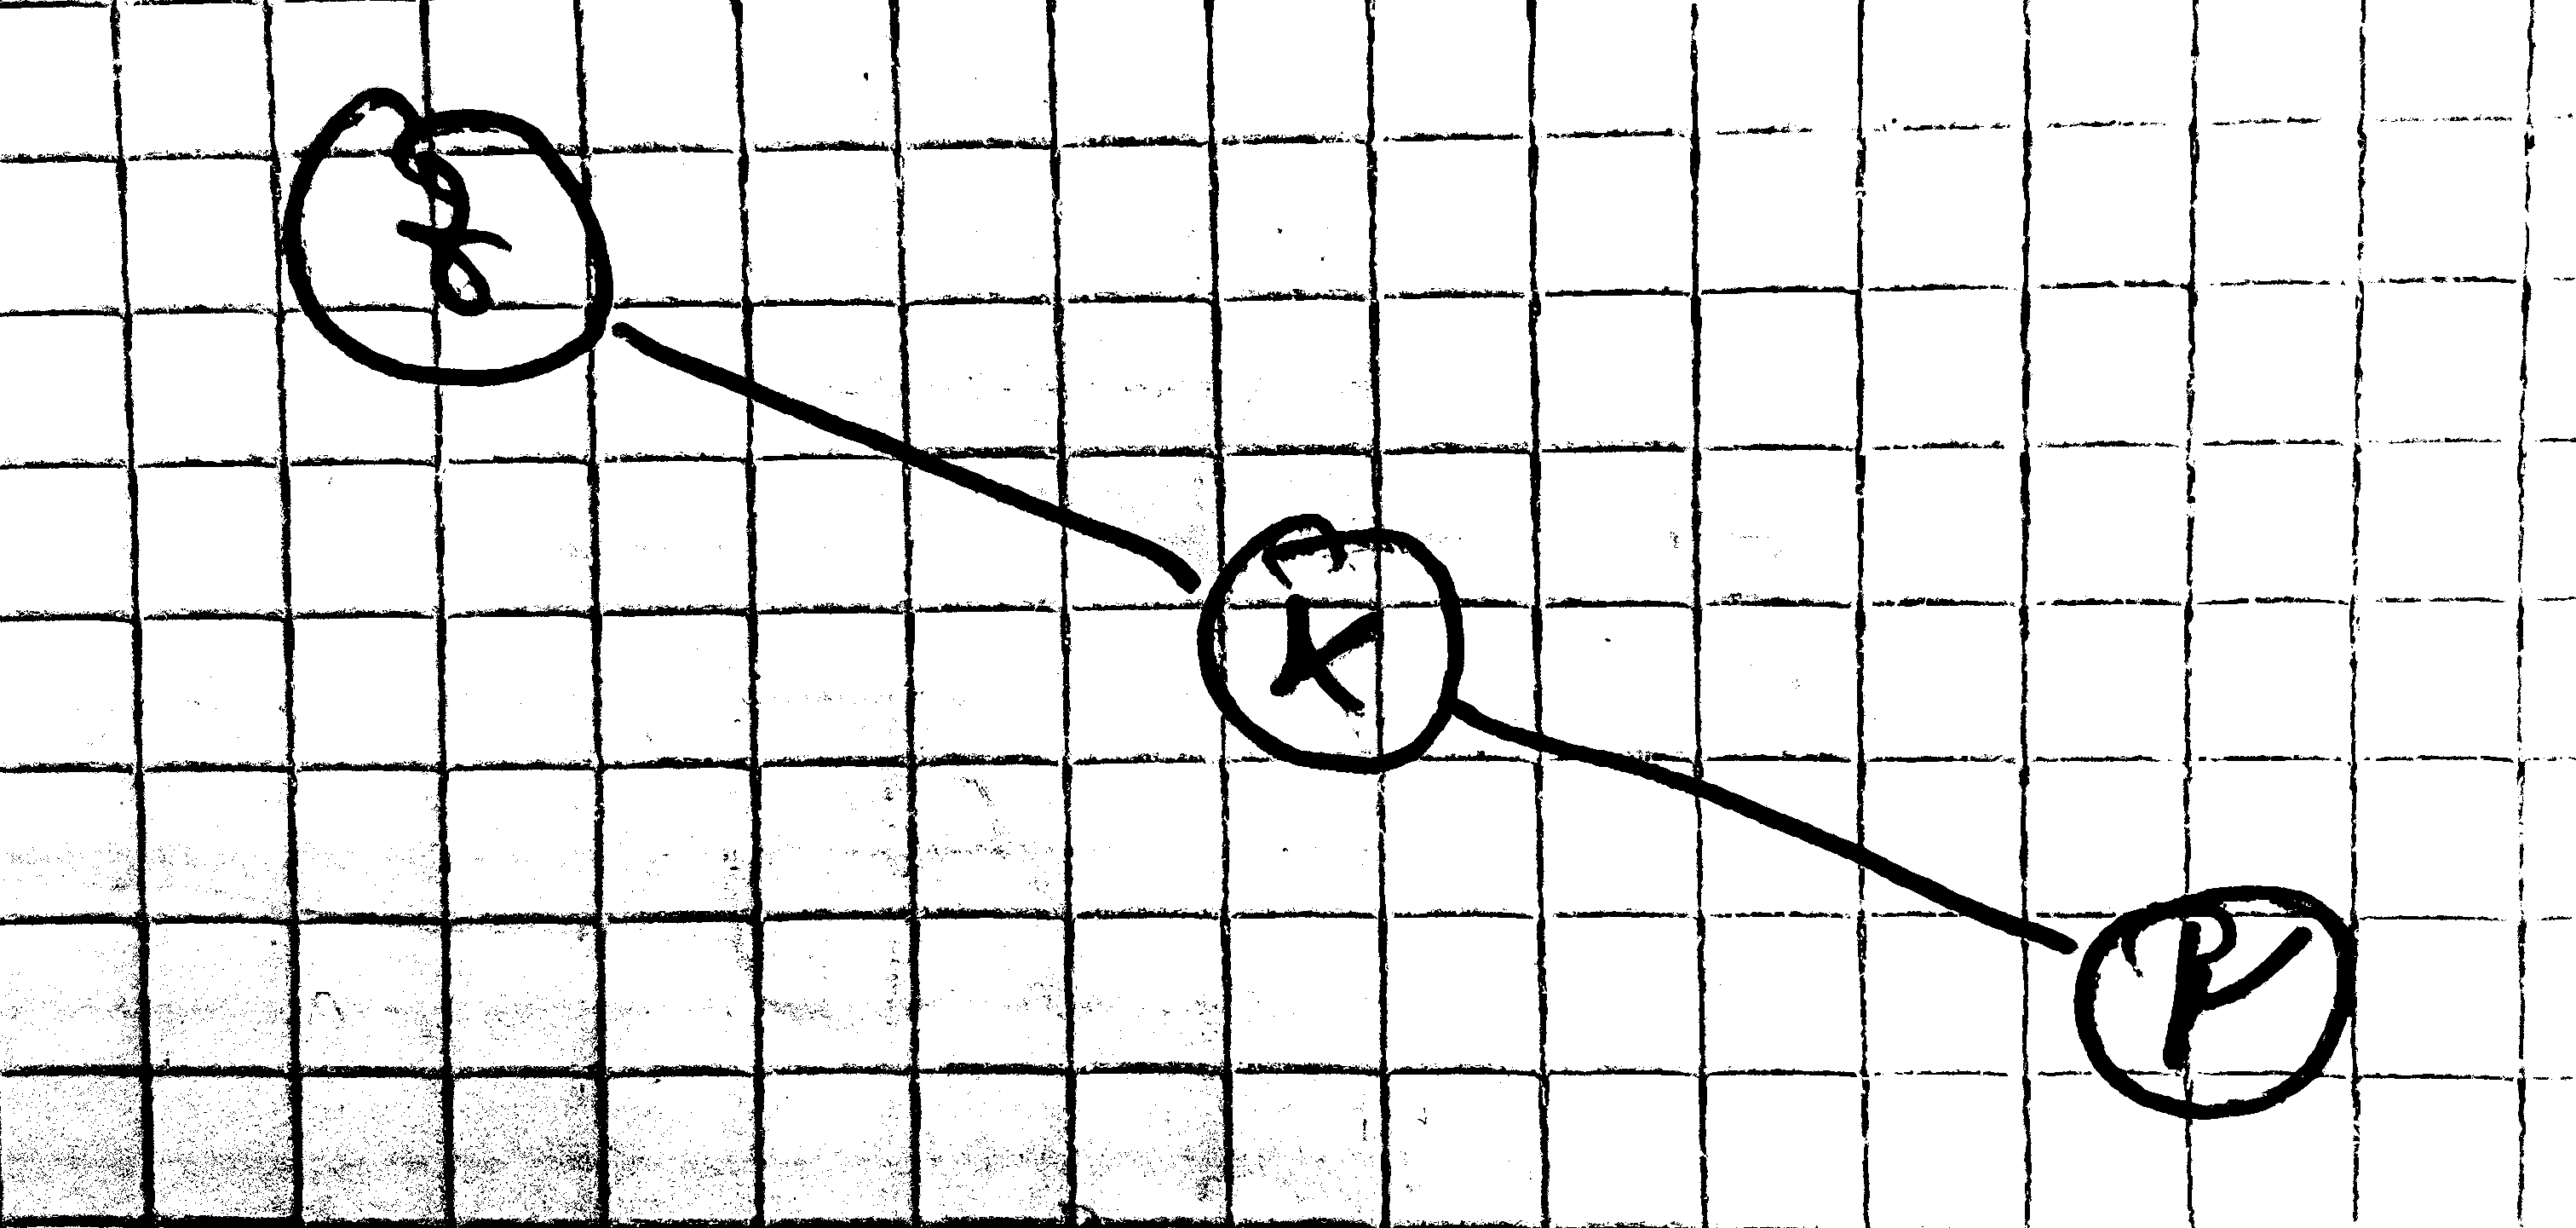
\includegraphics[scale=0.07]{imgs/img18.png}
	\end{center}
	\caption{X - истинная причина Y, если Z - потенциальная для X, и X блокирует путь из Z в Y}
	\label{fig:x_genuine_cause_of_y}
\end{figure}

\define{Случайная ассоциация} Две переменных $X, Y$ случайно ассоциированы, если они зависимы в каком-то контексте и существуют две другие переменные $Z_1, Z_2$ и два контекста $S_1, S_2$:

1. $X \not \independent Z_1 | S_1$

2. $Y \independent Z_1 | S_1$

3. $X \independent Z_2 | S_2$

4. $Y \not \independent Z_2 | S_2$

Условия 1 и 2 не позволяют назначить $X$ причиной $Y$: и правда, раз существует незаблокированный $S$ путь $Z_1 \leadsto X$, то не может оказаться, что $X$ - причина $Y$, ведь иначе был бы незаблокированный путь из $Z_1$ до $Y$  (\ref{fig:x_not_cause_of_y}). Аналогично условия 3,4 не позволяют назначить $Y$ потенциальной причиной $X$ (\ref{fig:y_not_cause_of_x}), что значит, что единственное объяснение их ассоциации - общая скрытая причина.

\begin{figure}[!tbph]
	\centering
	\begin{subfigure}[t]{0.4\textwidth}
		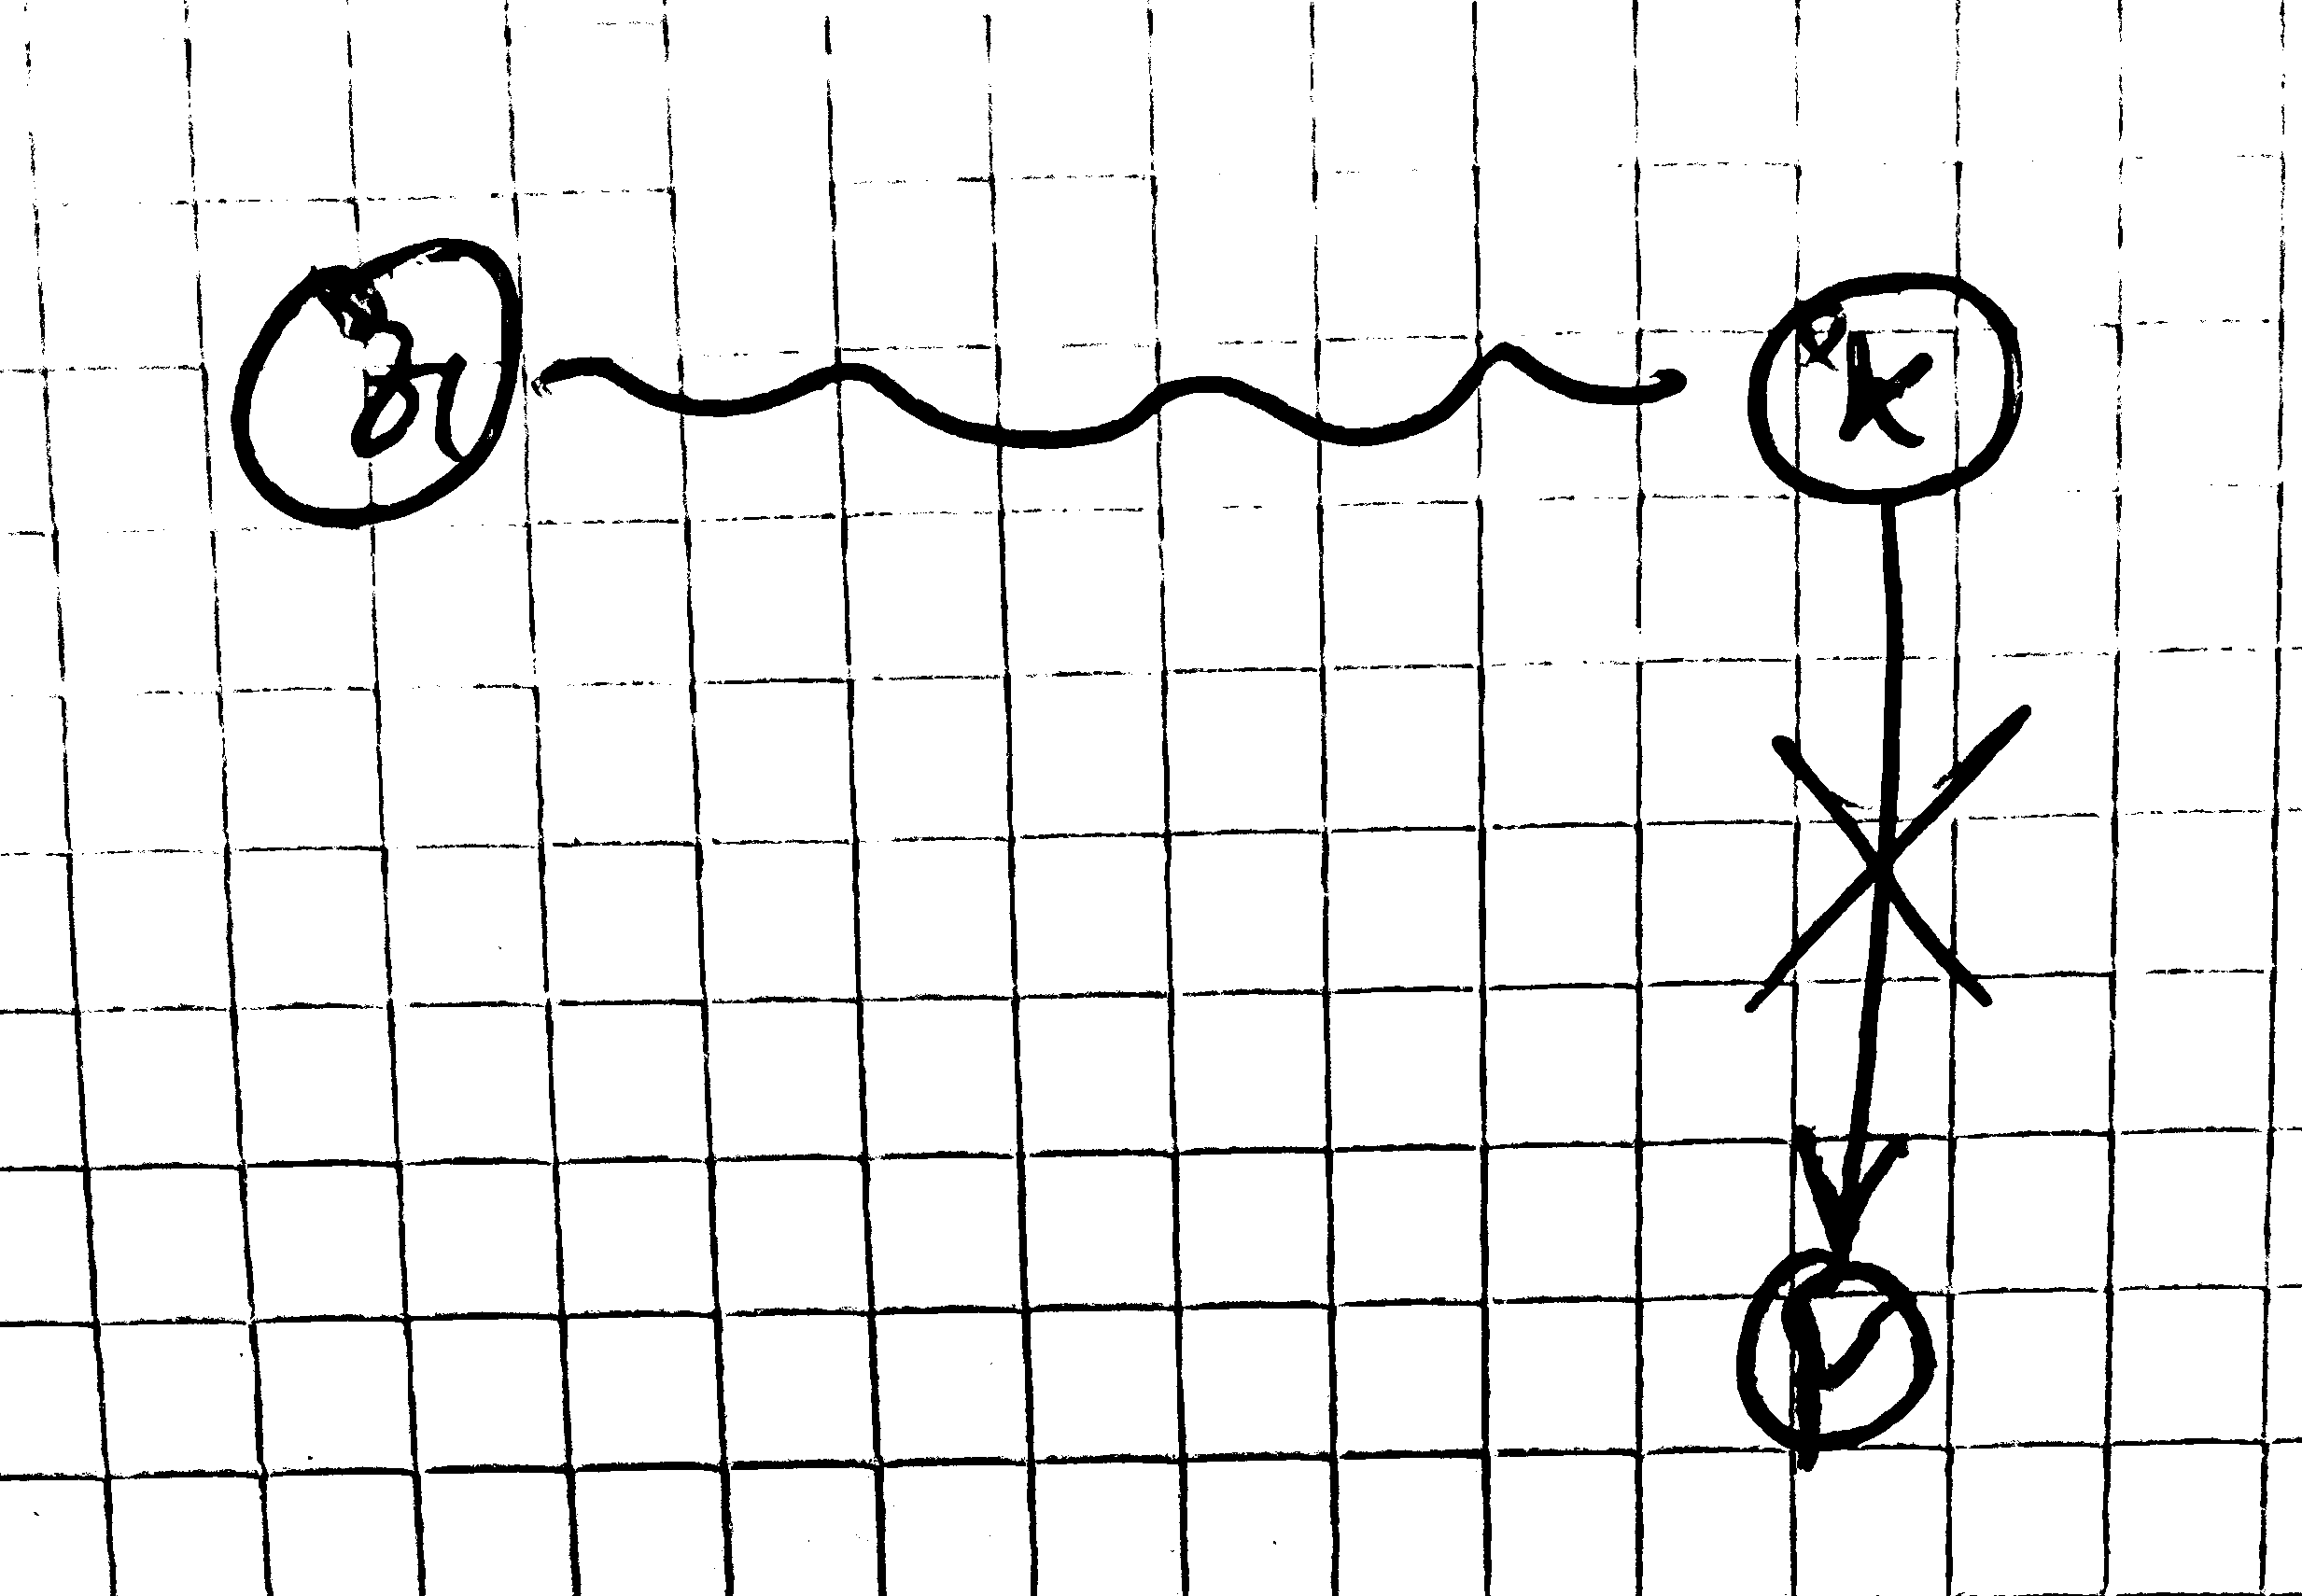
\includegraphics[width=\textwidth]{imgs/img15.png}
		\caption{X не может быть причиной Y}
		\label{fig:x_not_cause_of_y}
	\end{subfigure}
	\begin{subfigure}[t]{0.4\textwidth}
		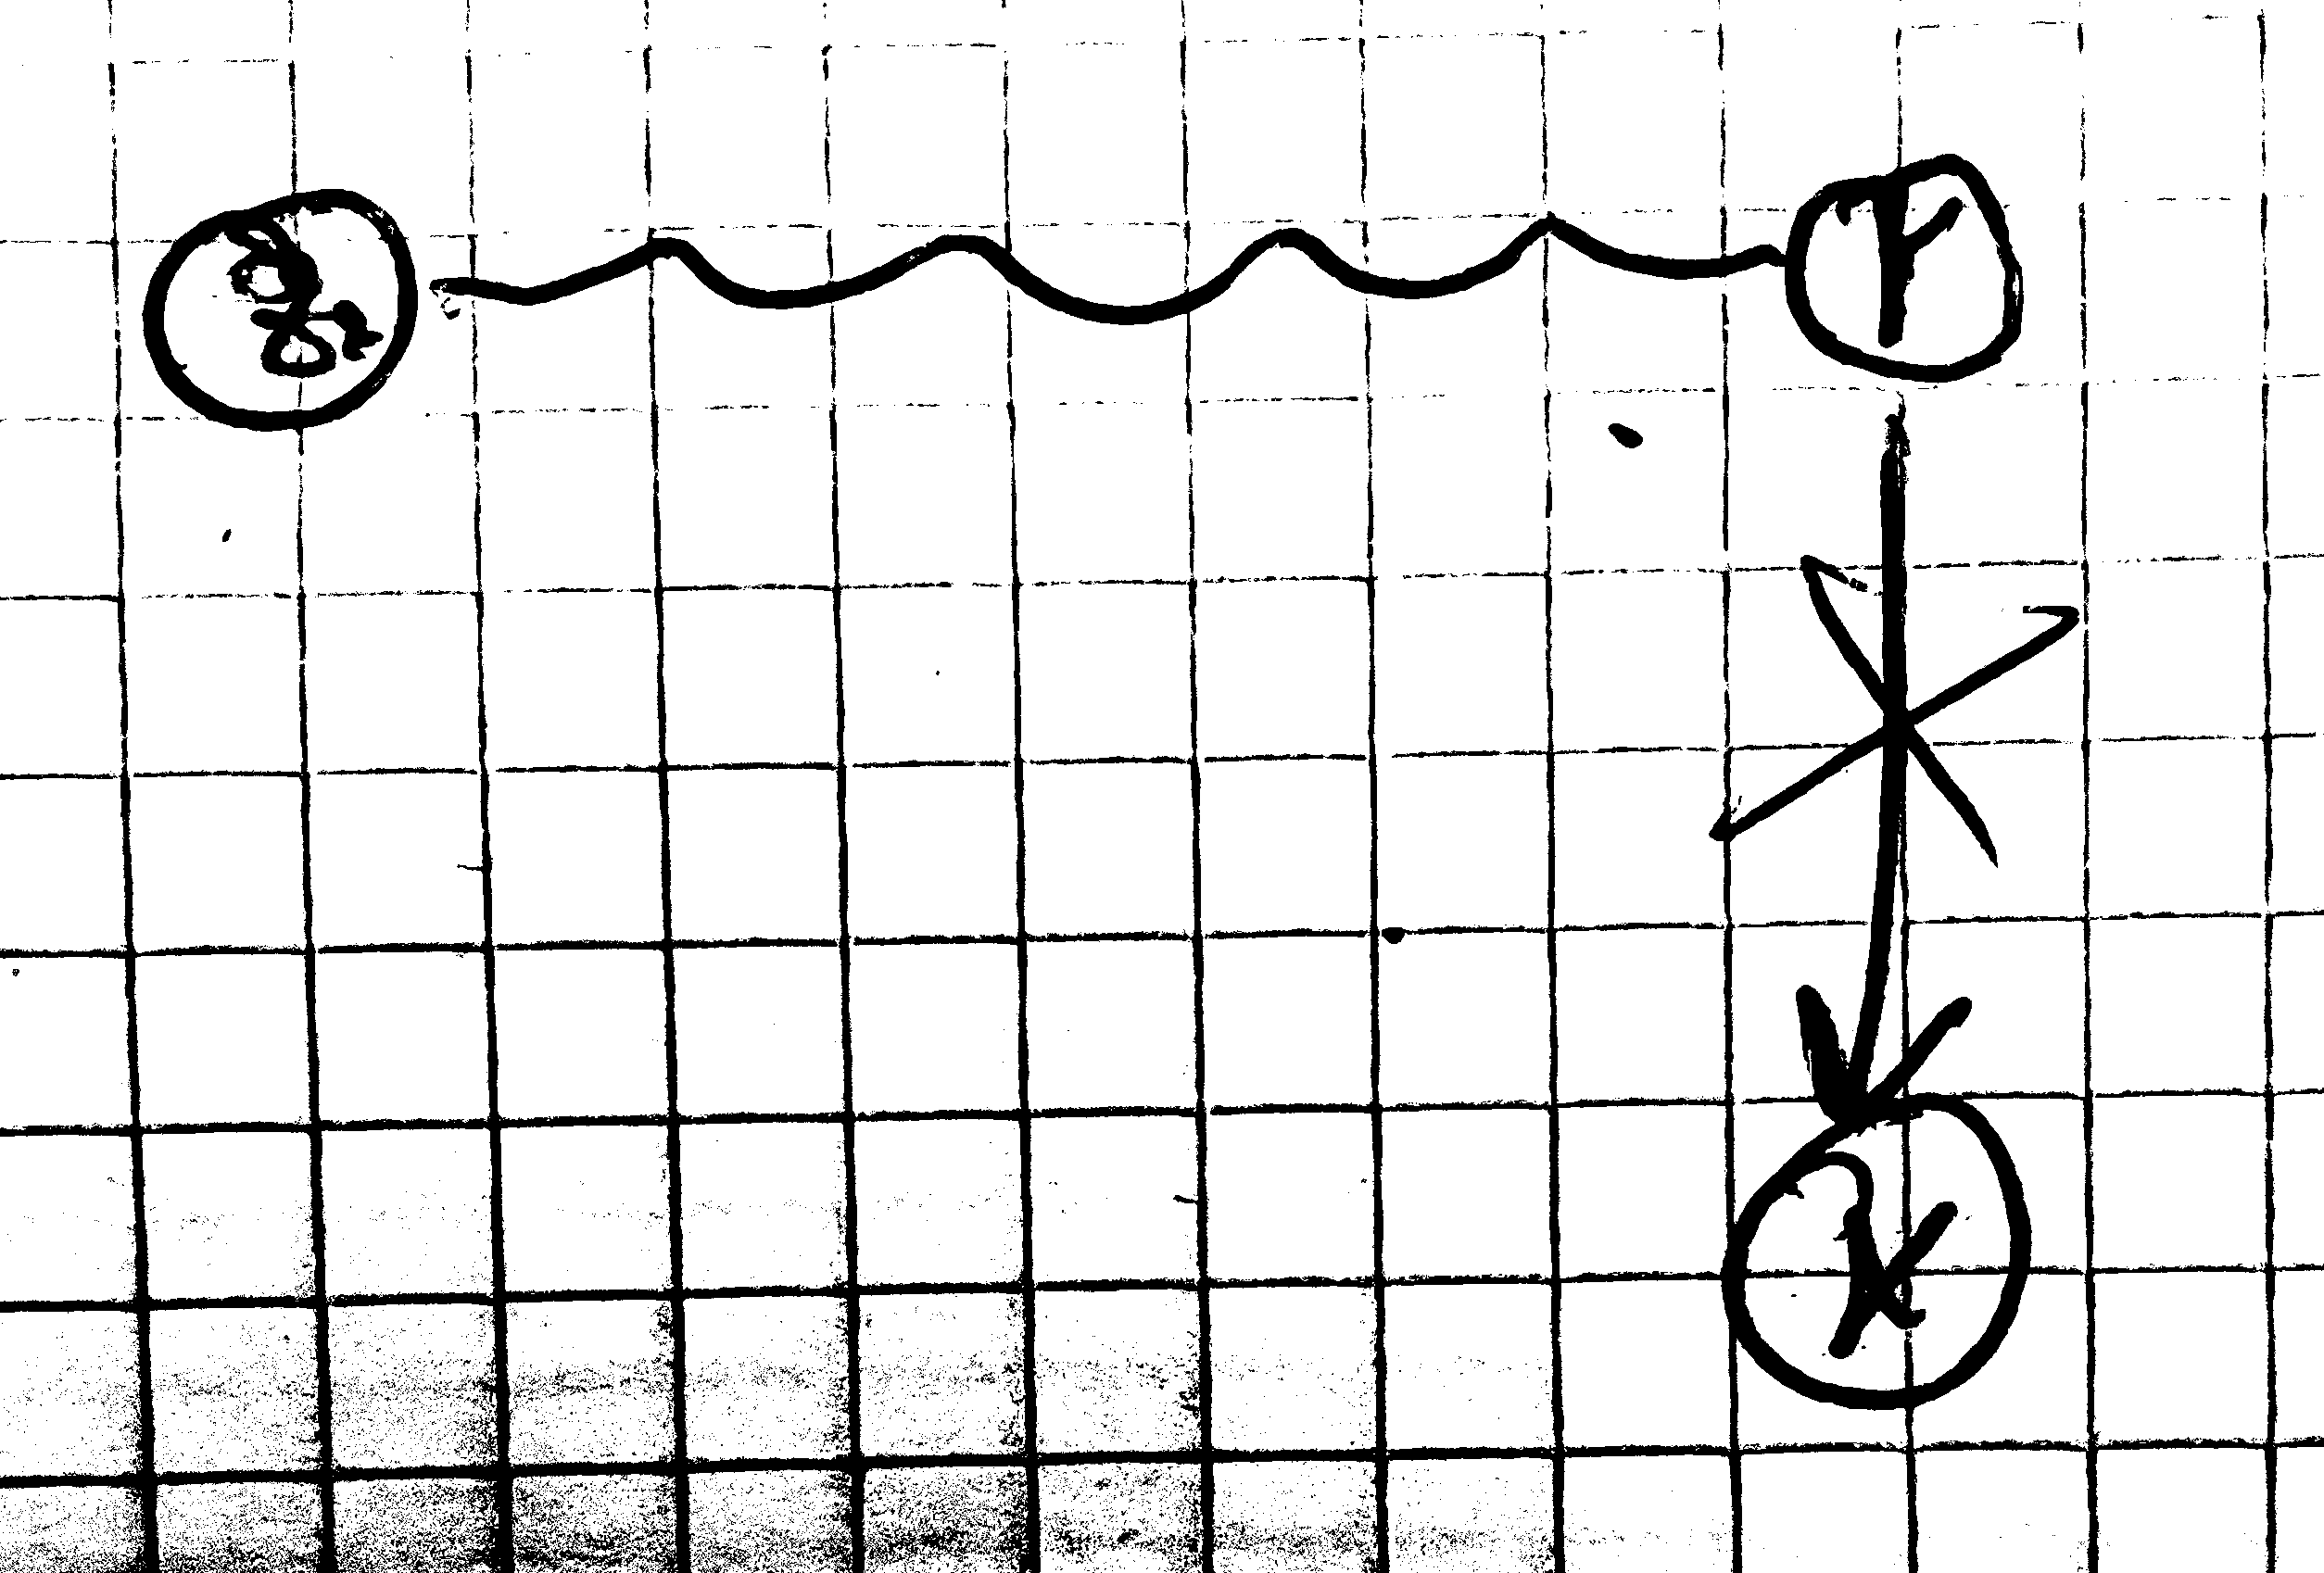
\includegraphics[width=\textwidth]{imgs/img16.png}
		\caption{Y не может быть причиной X}
		\label{fig:y_not_cause_of_x}
	\end{subfigure}
\end{figure}

Когда у нас появляется темпоральная информация, определение причинности упрощается: так, любое событие, которое предшествует другому, является его потенциальной причиной (ведь второе не может быть причиной первого, так как причина не может быть позднее следствия). Это приводит к более лаконичным определениям.

\define{Подлинная причина с темпоральной информацией} Переменная $X$ имеет подлинное причинное влияние на переменную $Y$, если существует контекст $S$ и переменная $Z$, произошедшие до $X$:

1. $Y \not \independent Z | S$

2. $Y \independent Z | S \cup X$

По сути, это всё то же определение подлинной причины без темпоральной информации, просто теперь для определения потенциальной причинности достаточно того, что $X$ случилось после $Z$.

\define{Случайная ассоциация с темпоральной информацией} - две переменные случайно ассоциированы, если $X$ произошла до $Y$, они зависимы в некотором контексте $S$, и существует переменная $Z$:

1. $Z \independent Y | S$

2. $Z \not \independent X | S$

\section{Причинные диаграммы и установление причинных эффектов}

В прошлой главе мы занимались тем, что изучали способы вывода причинных связей по сырым данным, без привлечения каких-либо дополнительных предположений. В этом же разделе мы будем изучать то, какие выводы можно сделать по комбинации данных и качественных причинных предположений, которые считаются приемлемыми в данном домене. Основной задачей будет выяснение, достаточно ли наблюдаемых данных (без необходимости проведения эксперимента) для выявления тех или иных причинных эффектов. 

Причинные эффекты позволяют понять, как система реагирует на интервенции. В этой главе для описания интервенций будем использовать причинные диаграммы, и определять постинтервенционные распределения через преинтервенционные. Мы покажем, что эффект любой интервенции может быть расчитан по исключительно наблюдаемым данным при условии, что в причинной диаграмме нет ненаблюдаемых переменных и эта диаграмма - DAG.

Когда не все переменные наблюдаемы возникает вопрос устанавливаемости причинных связей и эффектов. В этом разделе будет рассмотрен фреймворк для непараметрического выявления таких связей. 

\subsection*{Интервенции в марковских моделях}

\subsubsection*{Графы как модели интервенций}
Мы ранее установили, что причинные модели, в отличие от вероятностных, позволяют вычислять эффекты от интервенций. Для этого надо, чтобы совместное распределение $P$ было снабжено также причинной диаграммой - DAG, определяющим причинные связи между переменными. 

Самый простой тип интервенций - когда мы устанавливаем фиксированное значение $x_i$ какой-то переменной $X_i$. Такая интервенция, называемая атомарной, состоит в том, что $X_i$ перестаёт вести себя по закону, описанному в соответствующем функциональном уравнении $x_i = f_i(pa_i, u_i)$, а вместо этого ведёт себя по закону $x_i = x_i$ (тут слева $x_i$ это не константа, а просто обозначение переменной, знак равенства не симметричный в функциональных уравнениях). Для обозначения такой интервенции используют запись $do(X_i = x_i)$ или просто $do(x_i)$. В полученной новой модели (с замененным механизмом поведения $X_i$), если вычислить функцию распределения для $X_j$, можно получить причинный эффект $X_i$ на $X_j$, который обозначим $P(x_j | \hat x_i)$. 

В общем случае, когда интервенции подвергается множество переменных путем присвоения им фиксированных значений, мы удаляем соответствующие этим переменным уравнения, и получаем новое распределение, описывающее постинтервенционный мир.

\define{Причинный эффект (causal effect)} Пусть $X, Y$ - два непересекающихся множества переменных. Причинным эффектом $X$ на $Y$, обозначающимся $P(y|\hat x)$ или $P(y | do(x))$, называется функция, отображающая $X$ на пространство вероятностных распределений над $Y$. Для любой конкретной реализации $X = x$, $p(y|\hat x)$ определяет вероятность  $Y = y$ порожденную постинтервенционной причинной моделью. 

Как мы уже показывали ранее в разделе про причинные байесовские сети, граф, соответствующий усеченному множеству уравнений - это подграф исходного графа, в котором удалены все входящие рёбра в переменные, над которыми проведена интервенция. 

\subsubsection*{Интервенции как переменные}

В некоторых случаях удобно рассматривать возмущение, описывающее интервенцию, тоже как переменную в графе: то есть смотреть на $f_i$ как инстанс переменной $F_i$, и записывать структурное уравнение в виде 

\begin{align}
	\begin{split}
		x_i &= I(pa_i, f_i, u_i)
	\end{split}
\end{align}

Здесь I - некоторая трёхместная функция, удовлетворяющая условию $I(a,b,c)  \equiv f_i(a,c)$ если $b = f_i$. 

Соответствующая такой интерпретации интервенции диаграмма содержит новое ребро по сравнению с оригинальным графом:

\begin{figure}[h]
	\begin{center}
		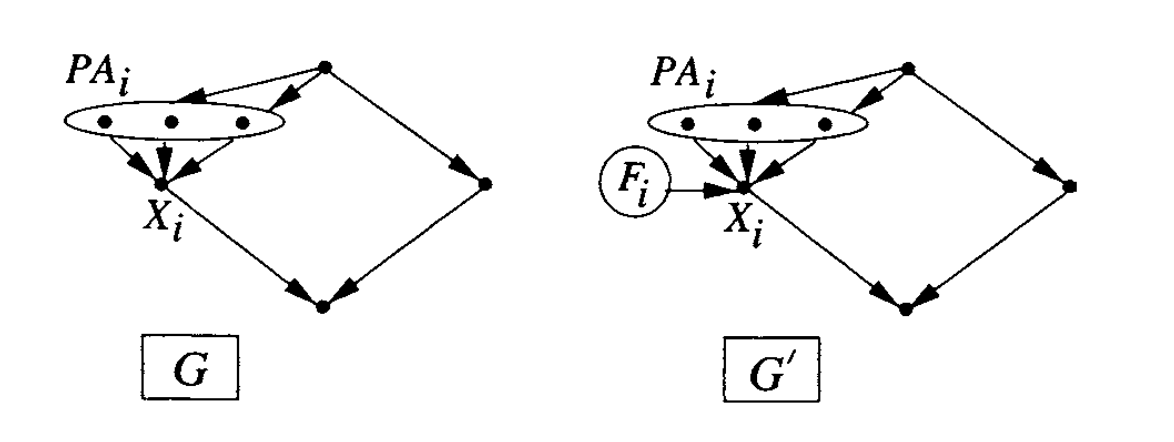
\includegraphics[scale=0.6]{imgs/img19.png}
	\end{center}
	\caption{Представление интервенции через расширенную диаграмму}
	\label{fig:explicit_intervention_in_graph}
\end{figure}

\subsubsection*{Вычисление эффекта интервенции}

Рассмотрим атомарную интервенцию $do(X_i = x_i')$. Она задаёт распределение $P(x_1,..,x_n|\hat x_i') = \prod\limits_{j\neq i}P(x_j | pa_j)$, когда $x_i = x_i'$, и равное 0 во всех остальных случаях. Разделим и умножим это равенство на $P(x_i | pa_i)$,  и получим 

\begin{align}
	P(x_1,...,x_n|\hat x_i') = \begin{cases}
		\frac{P(x_1,...,x_n)}{P(x_i | pa_i)} & \ x_i = x_i'\\
		0 & \ x_i \neq x_i'
		\end{cases}
	\label{eq:intervention}
\end{align}

На это равенство интересно посмотреть с точки зрения перераспределения масс: под действием интервенции, масса (вероятностная мера) точки  $(x_1, ..., x_n)$ возрастает в $\frac{1}{P(x_i' | pa_i)}$. Таким образом, для тех точек, для которых условная вероятность $P(x_i'|pa_i)$ мала, существенно увеличивают свою вероятность при интервенции, в то время как точки, для которых значение $X_i = x_i'$ довольно естественно ($P(x_i'|pa_i) \approx 1$) не сильно поменяют свою массу. 

В обычном байесовском подходе исключенные точки $x_i \neq x_i'$ переносят массу во все остальные точки посредством нормализационной константы $\frac{1}{P(x_i')}$. В нашем же случае происходит другая трансформация: масса точки распределяется между точками, шарящими с ней то же самое множество $pa_i$.  Действительно: $P(pa_i | do(x_i')) = P(pa_i)$ - то есть полная масса, распределенная по $pa_i$, сохраняется, а значит масса каждой точки $X = (s_i, x_i, pa_i)$, где $s_i = instance(S)$, $S = V \backslash (PA_i \cup \{X_i\})$ распределилась как-то между точками с тем же  $pa_i$ и $x_i = x_i'$. Коэффициент, на который увеличивается масса каждой точки, для данного $pa_i$ при этом один и тот же - $\frac{1}{P(x_i'|pa_i)}$.

Можно посмотреть на равенство \ref{eq:intervention} по-другому:

\begin{align}
	P(x_1,...,x_n|\hat x_i') = \begin{cases}
		P(x_1,...,x_n| x_i, pa_i)P(pa_i) & \ x_i = x_i'\\
		0 & \ x_i \neq x_i'
	\end{cases}
	\label{eq:intervention2}
\end{align}

\begin{theorem}
	\textbf{Учёт непосредственных причин}  Пусть $PA_i$ - множество непосредственных причин переменной $X_i$ и $Y \cap \{PA_i \cup X_i\} = \emptyset$. Тогда эффект интервенции $do(X_i = x_i')$ на $Y$ вычисляется по формуле 
	\begin{align}
		P(y|\hat x_i') = \sum\limits_{pa_i} P(y|x_i', pa_i) P(pa_i)
		\label{eq:adjusting_formula}
	\end{align}
\end{theorem}

Теорема следует непосредственно из суммирования формулы  \ref{eq:intervention2} по всем переменным кроме $Y$ $\blacksquare$.

Операция, состоящая в таком обуславливании с последующим усреднением результата, взвешенным априорными вероятностями $pa_i$, называется "поправкой на $PA_i$".

В более общем случае, когда интервенция состоит в установке какого-то подмножества переменных $S$ в константы $do(S = s)$, мы получаем аналогичную формулу для постинтервенционного распределения 

\begin{align}
	P(x_1,...,x_n|\hat s) = \begin{cases}
		\prod\limits_{i| X_i \notin S} P(x_i|pa_i) & x_1,...,x_n \text{ согласованное с} \  s\\
		0 & \text{иначе} 
	\end{cases}
\label{eq:intervention3}
\end{align}

Можно пойти ещё дальше, и рассмотреть произвольную интервенцию, заменяющую некоторые причинные механизмы на новые. Например, если заменить механизм, определяющий $X_i$: $P(x_i|pa_i) \leadsto P^*(x_i | pa^*_i)$ (может в том числе поменяться множество причин переменной $X_i$), то результирующее распределение после интервенции будет

\begin{align}
	P^*(x_1,..,x_n) = P(x_1,...,x_n) \frac{P^*(x_i|pa^*_i)}{P(x_i|pa_i)}
\end{align} 

Выводы: имея причинную диаграмму, в которой все непосредственные причины переменных, для которых проводится интервенция, были наблюдаемы, мы можем определить постинтервенционное распределение через преинтервенционное, используя формулу усеченной факторизации \ref{eq:intervention3}. 

Вообще говоря, интереснее ситуация, когда не все прямые причины наблюдаемы, что мешает непосредственному определению $P(x_i' | pa_i)$. Далее будут разработаны графические способы проверки того, можно ли оценить $P(x_j|\hat x_i')$, но для начала определим формально, что значит возможность оценить причинную величину  Q по пассивным наблюдениям - возможность \textit{идентификации}.

\subsubsection*{Идентификация причинных величин}

Причинные величины, в отличие от статистических параметров, определяются относительно причинной модели M, а не относительно одного лишь совместного распределения $P_M(v)$ над множеством наблюдаемых переменных. Так как неэкспериментальные данные дают информацию только о $P_M(v)$, и так как вообще говоря зачастую несколько моделей могут генерировать одно и то же распределение, существует возможность, что интересующая величина не будет однозначно определяться по имеющимся данным, причем независимо от того, как много семплов есть. Идентифицируемость гарантирует, что добавленные предположения о причинной модели (например, причинная структура или нулевые коэффициенты в структурных уравнениях) предоставят необходимые дополнительные сведения без необходимости задания модели M целиком. 

\define{Идентифицируемость} Пусть $Q(M)$ - любая вычисляемая величина в модели $M$. Мы говорим, что $Q(M)$ идентифицируема в классе моделей \textbf{M}, если для любых двух моделей из этого класса $M_1$ и $M_2$ оказывается $P_{M_1}(v) = P_{M_2}(v) \implies Q(M_1) = Q(M_2)$. Если наши наблюдения ограничены и мы знаем только некоторое множество фич $F_M$ распределения $P_M(v)$, то мы говорим, что $Q(M)$ идентифицируемо по $F_M$ если $F_{M_1} = F_{M_2} \implies Q(M_1) = Q(M_2)$.

Идентифицируемость необходима для объединения статистических данных с неполными причинными знаниями $\{f_i\}$, так как позволяет консистентно оценивать величины $Q$ по большим семплам $P(v)$ без детального определения $M$: достаточно некоторых общих характеристик класса моделей \textbf{M}. На данный момент, нас будет в качестве причинной величины $Q$ интересовать причинный эффект $P_M(y | \hat x)$, который конечно вычислим по заданной модели $M$ (используя его определение), но его обычно нам как раз надо вычислить, не имея полной спецификации модели $M$.

Мы будем рассматривать следующий класс \textbf{M} причинных моделей, внутри которого будем определять идентифицируемость:

1. Модели шарят общую причинную структуру

2. Определяют положительные распределения на множестве наблюдаемых переменных $v$: $P(v) > 0$.

\define{Идентифицируемость причинного эффекта} Причинный эффект $X$ на $Y$ идентифицируем из графа $G$, если величина $P(y|\hat x)$ может быть однозначно вычислена из любого положительного распределения наблюдаемых переменных, то есть если $P_{M_1}(y|\hat x) = P_{M_2}(y|\hat x)$ для любой пары моделей $M_1, M_2$, для которых $P_{M_1}(v) = P_{M_2}(v)$ и графы которых совпадают.

Идентифицируемость $P(y|\hat x)$ гарантирует, что причинный эффект $do(X = x)$ на $Y$ можно вычислить по двум источникам данных:

1. Пассивным наблюдениям, позволяющим восстановить $P(v)$

2. Причинному графу $G$, который определяет (качественно), какие переменные задают стабильные причинные механизмы (какие переменные определяют другие переменные).

Положительность распределения гарантирует то, что в формуле \ref{eq:intervention} мы не будем делить на 0: логично, если бы вероятность наблюдать $x_i'$ в контексте $pa_i$ была нулевой, мы бы не смогли вывести эффект от действия $do(X_i=x_i')$. 

Отметим, чтобы установить неидентифицируемость, достаточно предоставить в качестве примера два множества структурных уравнений, задающих одинаковые распределения над наблюдаемыми переменными, но имеющих различные причинные эффекты.

\begin{theorem}
	При заданной причинной диаграмме G любой марковской модели, в которой некоторое подмножество V переменных наблюдаемо, причинный эффект $P(y|\hat x)$ идентифицируем если $\{X \cup Y \cup PA_x\} \subset V$. Выражение для $P(y|\hat x)$ в этом случае определяется путем учёта непосредственных причин по формуле \ref{eq:adjusting_formula}.
\end{theorem}

\subsection*{Контроль путающего смещения (confounding)}

Когда мы хотим оценить эффект какого-то фактора $X$ на другой $Y$, возникает вопрос нужно ли нам стандартизировать измерения на различные значения прочих факторов $Z$, также известных как ковариации/конфаундеры. Стандартизация состоит в разбиении популяции на подгруппы, которые гомогенны относительно значения $Z$, затем оценивании эффекта в каждой подгруппе и усреднение результата. 

Иллюзорная природа стандартизации была обнаружена еще пирсоном в 1899, когда он обнаружил парадокс Симпсона: любая статистическая связь между двумя переменными может быть инвертирована путем включения дополнительных факторов в анализ. Соответственно встаёт вопрос - какие переменные нам следует учитывать во избежание конфаундинга? 

\subsubsection*{Критерий задней двери}

\define{Backdoor criterion} Множество переменных $Z$ удовлетворяет критерию задней двери относительно упорядоченной пары переменных $(X_i, X_j)$ в DAG G если 

1. Никакая вершина в $Z$ не является наследником $X_i$

2. $Z$ блокирует любой путь между $X_i$ и $X_j$, в котором есть ребро, направленное в $X_i$

В общем случае, когда есть два множества переменных $X, Y$, говорят что $Z$ удовлетворяет критерию задней двери, если оно удовлетворяет ему для любой упорядоченной пары $(X_i, X_j): X_i \in X, X_j \in Y$


\begin{theorem}
	\textbf{Поправка задней двери} Если множество переменных $Z$ удовлетворяет критерию задней двери относительно $(X,Y)$, то причинный эффект идентифицируем и задаётся формулой 
	
	\begin{align}
		P(y|\hat x) = \sum\limits_{z} P(y|x, z) P(z)
	\end{align}
\end{theorem}

Докажем теорему. Для доказательства удобнее всего рассматривать расширенный граф, в котором представлены вершины, задающие причинные механизмы. Раз все заднедверные пути заблокированы $Z$, то любой путь, $F_x \leadsto Y$ идет через детей $X$, но эти пути заблокированы при обуславливании на $X$. В итоге, мы приходим к тому, что $Y$ независимо от $F_x$ при условии $X, Z$:

\begin{align}
P(y|x, z, F_x = do(x)) = P(y | x, z, F_x = idle) = P(y|x, z)
\label{eq:backdoor1}
\end{align}
что означает, что наблюдение $X=x$ неотличимо в контексте $Z$ от интервенции $do(X = x)$.

Действительно,  если $P'$ - распределение, порожденное расширенным графом $G'$, то

\begin{align}
	P(y|\hat x) = P'(y|F_x) = \sum\limits_{z}P'(y|z, F_x)P'(z|F_x) = \sum\limits_{z}P'(y|z, x, F_x)P'(z|F_x)
\end{align}

Последнее равенство верно, так как $F_x \implies X = x$. Теперь нам остается избавиться от двух $F_x$ в правой части равенства. Заметим, что $F_x$ - это корневые вершины в $G'$, с детьми $X$. Поэтому, $F_x \independent Z | X$, так как они d-отделены, ведь $Z$ - не наследники $X$ по первому пункту бэкдор критерия. Поэтому

\begin{align}
	P'(z|F_x) = P'(z) = P(z)
\end{align}

Что касается $P'(y|z, x, F_x)$, то согласно \ref{eq:backdoor1} оно эквивалентно $P(y|x,z)$.  В итоге, мы получаем ровно то, что и требовалось. $\blacksquare$

\subsubsection*{Фронтальный критерий}

Рассмотрим следующую диаграмму:
\begin{figure}[h]
	\begin{center}
		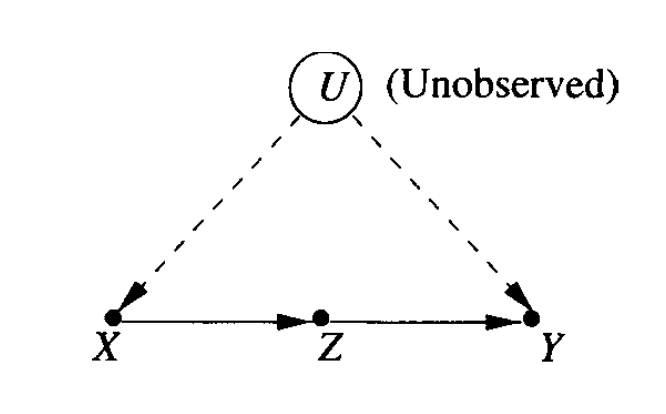
\includegraphics[scale=0.6]{imgs/img20.png}
	\end{center}
	\caption{Диаграмма для представления фронтального критерия}
	\label{fig:frontdoor1}
\end{figure}

Соответствующее диаграмме распределение факторизуется согласно 

\begin{align}
	P(x,z,y,u) = P(u)P(x|u)P(z|x)P(y|z,u)
\end{align}

Интервенция $X=do(x)$ приводит нас к факторизации без множителя для $X$:

\begin{align}
	P(z,y,u|\hat x) = P(u)P(z|x)P(y|z,u)
\end{align}

Просуммируем по $u,z$ для вычисления эффекта на $y$:

\begin{align}
	P(y|\hat x) = \sum\limits_{z}P(z|x)\sum\limits_{u}P(u)P(y|z,u)
	\label{eq:frontdoor2}
\end{align}

Этим просто так не воспользоваться, так как у нас $u$ ненаблюдаемая - от неё надо как-то избавиться. 

Заметим, что по d-разделению в графе имеем следующие независимости:

\begin{align}
	P(u|z,x) = P(u|x)\label{eq:frontdoor_cond1}\\
	P(y|z,u,x) = P(y|u,z)
	\label{eq:frontdoor_cond2}
\end{align}

Используя эти равенства, рассмотрим компонент \ref{eq:frontdoor2}
\begin{align}
	\begin{split}
	\sum\limits_{u}P(u)P(y|z,u) &= \sum\limits_{x} \sum\limits_{u}P(u|x)P(x)P(y|z,u)\\ 
	&= \sum\limits_{x} \sum\limits_{u}P(u|x,z)P(x)P(y|z,u,x) \\
	&= \sum\limits_{x} \sum\limits_{u}P(y,u|z,x)P(x) \\
	&= \sum\limits_{x} P(y|z,x)P(x)
	\end{split}
	\label{eq:frontdoor3}
\end{align}

что позволяет нам преобразовать \ref{eq:frontdoor2} в 
\begin{align}
	P(y|\hat x) = \sum\limits_{z}P(z|x) \sum\limits_{x} P(y|z,x)P(x)
	\label{eq:frontdoor4}
\end{align}

В данной формуле все множители в правой части могут быть оценены по наблюдаемым данным, из чего следует, что $P(y|\hat x)$ так же можно оценить. Таким образом, при условии что $Z$  удовлетворяет \ref{eq:frontdoor_cond1}, \ref{eq:frontdoor_cond2} мы можем несмещенно оценить эффект $X$ на $Y$.

Формулу \ref{eq:frontdoor4} можно интерпретировать как двухшаговое применение бэкдор-выравнивания: первым шагом мы вычисляем эффект $X$ на $Z$: так как нет ни одного разблокированного бэкдор-пути из $Z$ в $X$, то 

\begin{align}
	P(z|\hat x) = P(z|x)
\end{align}

Затем, мы вычисляем эффект $Z$ на $Y$. Тут у нас уже есть незаблокированный бэкдор-путь $Y \leftarrow U \rightarrow X \rightarrow Z$, который однако можно заблокировать, обусловившись на $X$, так что $X$ удовлетворяет в данном случае бэкдор-критерию и потому 

\begin{align}
	P(y|\hat z) = \sum\limits_{x'}P(y|z,x')P(x')
\end{align}

В итоге, мы комбинируем два причинных эффекта чтобы получить
\begin{align}
	P(y|\hat x) = \sum\limits_{z}P(z|\hat x) P(y|\hat z)
\end{align}

\define{Фронтальный критерий}
Множество переменных $Z$ удовлетворяет фронтальному критерию относительно упорядоченной пары переменных ($X$,$Y$), если 

1. Z блокирует все направленные пути $X \leadsto Y$

2. Нету незаблокированного бэкдор-пути $Z \leadsto X$

3. Все бэкдор-пути $Y \leadsto Z$ заблокированы $X$. 

\begin{theorem}
	\textbf{Фронтальная корректировка} Если $Z$ удовлетворяет фронтальному критерию относительно $(X, Y)$ и $P(x,z) > 0$, то причинный эффект $X$ на $Y$ идентифицируем и может быть вычислен как 
	\begin{align}
		P(y|\hat x) = \sum\limits_{z}P(z|x) \sum\limits_{x'}P(y|z,x')
	\end{align}
	 
\end{theorem}


\end{document}